\documentclass[12pt]{article}

\setlength{\oddsidemargin}{0in}
\setlength{\textwidth}{\paperwidth}
\addtolength{\textwidth}{-2in}
\setlength{\topmargin}{-.5in}
\setlength{\textheight}{8.75in}
\usepackage{amsmath,amssymb,amsthm,color,epsfig,mathrsfs}
\usepackage{amsbsy}
%\usepackage{esint}
%\usepackage{txfonts}
%\usepackage{pxfonts}
%\pagestyle{empty}

\usepackage{tabularx,ragged2e,booktabs,caption}
%\usepackage{showkeys}  % SHOW LABELS

%\renewcommand{\thesection}{{\arabic{section}}}
%\renewcommand{\thesection}{}
%\renewcommand{\thesubsection}{}

%\newcommand{\tmpsection}[1]{}
%\let\tmpsection=\section
%\renewcommand{\section}[1]{\tmpsection{\centerline{\hspace*{-2em}\arabic{section}. #1}}}

%\newcommand{\tmpsubsection}[1]{}
%\let\tmpsubsection=\subsection
%\renewcommand{\subsection}[1]{\tmpsubsection{\itshape\hspace*{-1em}\arabic{section}.\arabic{subsection} #1}}

\renewcommand{\theequation}{\arabic{section}{.}\arabic{equation}}

\renewcommand{\labelitemi}{{\begin{picture}(1,1)
     \setlength{\unitlength}{0.5cm}
     \put(0,0.22){\circle*{0.2}}
    \end{picture}}}

%\usepackage{epsfig}
%\usepackage{graphicx}
%\usepackage{mathrsfs}

%\usepackage[english,french]{babel}
%\selectlanguage{french} 

%\usepackage[T1]{fontenc}
%\usepackage[latin1]{inputenc}

%\usepackage{amsthm}
%\usepackage{amsmath,amssymb,amsbsy,color}
%\usepackage{showkeys}


% Permet de num?roter les ?quations par section
%\renewcommand{\theequation}{{\arabic{section}.\arabic{equation}}}

\newtheorem{theorem}{Theorem}
\newtheorem{acknowledgement}[theorem]{Acknowledgement}
\newtheorem{algorithm}[theorem]{Algorithm}
\newtheorem{axiom}[theorem]{Axiom}
\newtheorem{case}[theorem]{Case}
\newtheorem{claim}[theorem]{Claim}
\newtheorem{conclusion}[theorem]{Conclusion}
\newtheorem{condition}[theorem]{Condition}
\newtheorem{conjecture}[theorem]{Conjecture}
\newtheorem{corollary}[theorem]{Corollary}
\newtheorem{criterion}[theorem]{Criterion}
\newtheorem{principle}[theorem]{Rule}
\newtheorem{definition}[theorem]{Definition}
\newtheorem{example}[theorem]{Example}
\newtheorem{exercise}[theorem]{Exercise}
\newtheorem{lemma}[theorem]{Lemma}
\newtheorem{notation}[theorem]{Notation}
\newtheorem{problem}[theorem]{Problem}
\newtheorem{proposition}[theorem]{Proposition}
\newtheorem{remark}[theorem]{Remark}
\newtheorem{solution}[theorem]{Solution}
\newtheorem{summary}[theorem]{Summary}
%\newenvironment{proof}[1][Proof]{\noindent\textbf{#1.} }{\ \rule{0.5em}{0.5em}}

% My list environment
\newcounter{spslist}
\newenvironment{spslist}{
  \begin{list}
  {\begin{picture}(1,1)
     \setlength{\unitlength}{0.5cm}
     \put(0,0.22){\circle*{0.2}}
    \end{picture}}
  {\usecounter{spslist}
  \setlength{\leftmargin}{1em}
  \setlength{\labelsep}{0.6em}
  \setlength{\labelwidth}{1em}
  \setlength{\topsep}{1ex}
  \setlength{\rightmargin}{0em}
  \setlength{\itemsep}{0.5ex}
  \setlength{\parsep}{0em}
  \setlength{\itemindent}{0em} }}
  {\end{list}}

\newcommand{\col}[3]{ \renewcommand{\arraystretch}{#1}
                \left[\!\! \begin{array}{c} #2 \\ #3 \end{array} \!\!\right] }
\newcommand{\row}[3]{ \renewcommand{\arraystretch}{#1}
                \left[\! \begin{array}{cc} #2 & #3 \end{array} \!\right] }
\newcommand{\mat}[5]{ \renewcommand{\arraystretch}{#1}
                    \left[\! \begin{array}{cc}
                            #2 & #3 \\
                            #4 & #5 \end{array} \!\right] }
%\newcommand{\col}[2]{\left( \!\! \begin{array}{c} #1 \\ #2 \end{array} \!\! \right)}
%\newcommand{\mat}[4]{\left( \!\! \begin{array}{cc} #1 & #2 \\ #2 & #4 \end{array} \!\! \right)}

%%%%%%%%%%%%%%%%%%%%
\newcounter{geqncount}
\newenvironment{groupeqn}%
    {\refstepcounter{equation}%
     \setcounter{geqncount}{\value{equation}}%
     \setcounter{equation}{0}%
  \renewcommand{\theequation}{\arabic{section}.\arabic{geqncount}.\alph{equation}}}%
    {\setcounter{equation}{\value{geqncount}}}
%%%%%%%%%%%%%%%%%%%%

%\numberwithin{equation}{section}


\newcommand{\eps}{\epsilon}
\newcommand{\half}{{\textstyle{\frac{1}{2}}}}
\newcommand{\fourth}{{\textstyle{\frac{1}{4}}}}

%    SPECIAL NOTATION FOR FIELDS AND FRIENDS    %%%%%%%%%%%%%%%%%%%

\newcommand{\CC}{\mathbb{C}}
\newcommand{\RR}{\mathbb{R}}
\newcommand{\ZZ}{\mathbb{Z}}
\newcommand{\cchi}[1]{{\textstyle{\chi\big(#1\big)}}}
\newcommand{\Dmax}{\mathcal{D}_+}
\newcommand{\Dmin}{\mathcal{D}_-}
\newcommand{\Daux}{\mathcal{D}_\text{\!aux}}
\newcommand{\Dloc}{\mathcal{D}_\text{\!loc}}
\newcommand{\Hmax}{H_+}
\newcommand{\Hmin}{H_-}
\newcommand{\Nplus}{{\mathcal N}_i}
\newcommand{\Nminus}{{\mathcal N}_{-i}}
\newcommand{\Nlambda}{{\mathcal N}_\lambda}
\newcommand{\Alambda}{{\mathcal A}_\lambda}
\newcommand{\supp}{\mathrm{supp}}
\newcommand{\Hloc}{H^2_\text{loc}}
\newcommand{\Hstar}{H^2_*}

% NOTES

\newcommand{\notejt}[1]{{\color[rgb]{0,0,1.0}[#1]}}
\newcommand{\notesps}[1]{{\color[rgb]{1,0.5,0}[#1]}}

\bibliographystyle{plain}


\begin{document}


\bibliographystyle{plain} % Choose Phys. Rev. style for bibliography



\begin{center}
{\bfseries \Large  Spectra of half-infinite quantum graph tubes}
\end{center}

\vspace{0ex}

\begin{center}
{\scshape \large Stephen P. Shipman \,and\, Jeremy Tillay\\
\vspace{2ex}
{
\itshape
Department of Mathematics\\
Louisiana State University\\
Baton Rouge, Louisiana \ 70803, USA
}}
\end{center}

\vspace{3ex}
\centerline{\parbox{0.9\textwidth}{
{\bf Abstract.}\
cARBON nanotubes yay
}}

\vspace{3ex}
\noindent
\begin{mbox}
{\bf Key words:}
quantum graph, spectrum, embedded eigenvalue, nanotube, self-adjoint extensions
\end{mbox}
\vspace{3ex}

\hrule
\vspace{1.1ex}



\section{Introduction} %%%%%%%%%%%%%%%%%%%%%%%%%%%%%%%%%%%

A quantum graph is a metric graph (a set of vertices and edges where each edge is parametrized by an interval ) equipped with a schrodinger operator that acts on functions defined along the edges of the graph. Consider a two-dimensional square lattice, treated as a quantum graph equipped with the second derivative operator 
$ H= \partial xx \ $, which is a schrodinger operator with a zero potential. 

Now we consider the property of self-adjointness. This operator H is self-adjoint with respect to the domain of functions if the the following equality $<Hu, v> \ = \ <u, Hv>$ holds for all functions within the specified domain. Note that the inner product of two functions u and v is considered here to be the $L^2[0, 1]$ norm acting on functions in $H^2[0, 1]$:

\centerline{\scalebox{0.3}{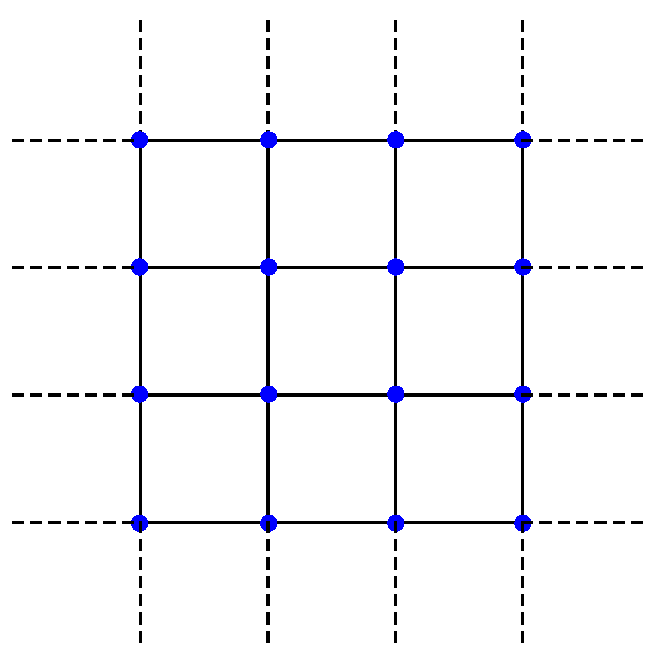
\includegraphics{squarelattice.pdf}}}
  
(Talk about self-adjointness requiring me to restrict domain of functions using vertex conditions. Discuss what our inner product space is. I'm in H2 with L2 inner product and vertex conditions) 

$<u, v> = \sum\nolimits_{e \in Q} \int_{0}^{1}u*v$

So in order for the second-derivative operator H to be self-adjoint, it must be that $<Hu, v> = <u, Hv> $

Or equivalently

$\sum\nolimits_{e \in Q} \int_{0}^{1}u''*v= \sum\nolimits_{e \in Q} \int_{0}^{1}v''*u$

\section{Eigenmodes of the infinite tube} %%%%%%%%%%%%%%%%%%%%%%%%%%%%%%%%%%%

... ...


\subsection{Some notation}

The standard (Neumann) vertex condition ...

Some domains of Schr\"odinger operators, as subspaces of $L^2$ ...

For a metric graph $\Gamma$, define a local $H^2$ space with unspecified conditions at pendant vertices:
%
\begin{equation}
  \Hloc(\Gamma) = \big\{ u\in \bigoplus\limits_{e\in E(\Gamma)} H^2(e)
                                    \,:\,  \text{$u$ satisfies the standard condition at each internal vertex}  \big\}
\end{equation}
%
This space is contained in a larger one, in which only continuity is required at internal vertices:
%
\begin{equation}
  \Hstar(\Gamma) = \big\{ u\in \bigoplus\limits_{e\in E(\Gamma)} H^2(e)
                                    \,:\,  \text{$u$ is continuous at each internal vertex}  \big\}
\end{equation}
%


Schr\"odinger operators on these spaces ...



\subsection{A square-periodic quantum graph}

... ... (Fig~\ref{fig:FundamentalDomain}).

\begin{figure}  %%%%%%%%%%%%%%%%% FIGURE %%%%%%%%%%%%%%%%%%
\centerline{\scalebox{0.3}{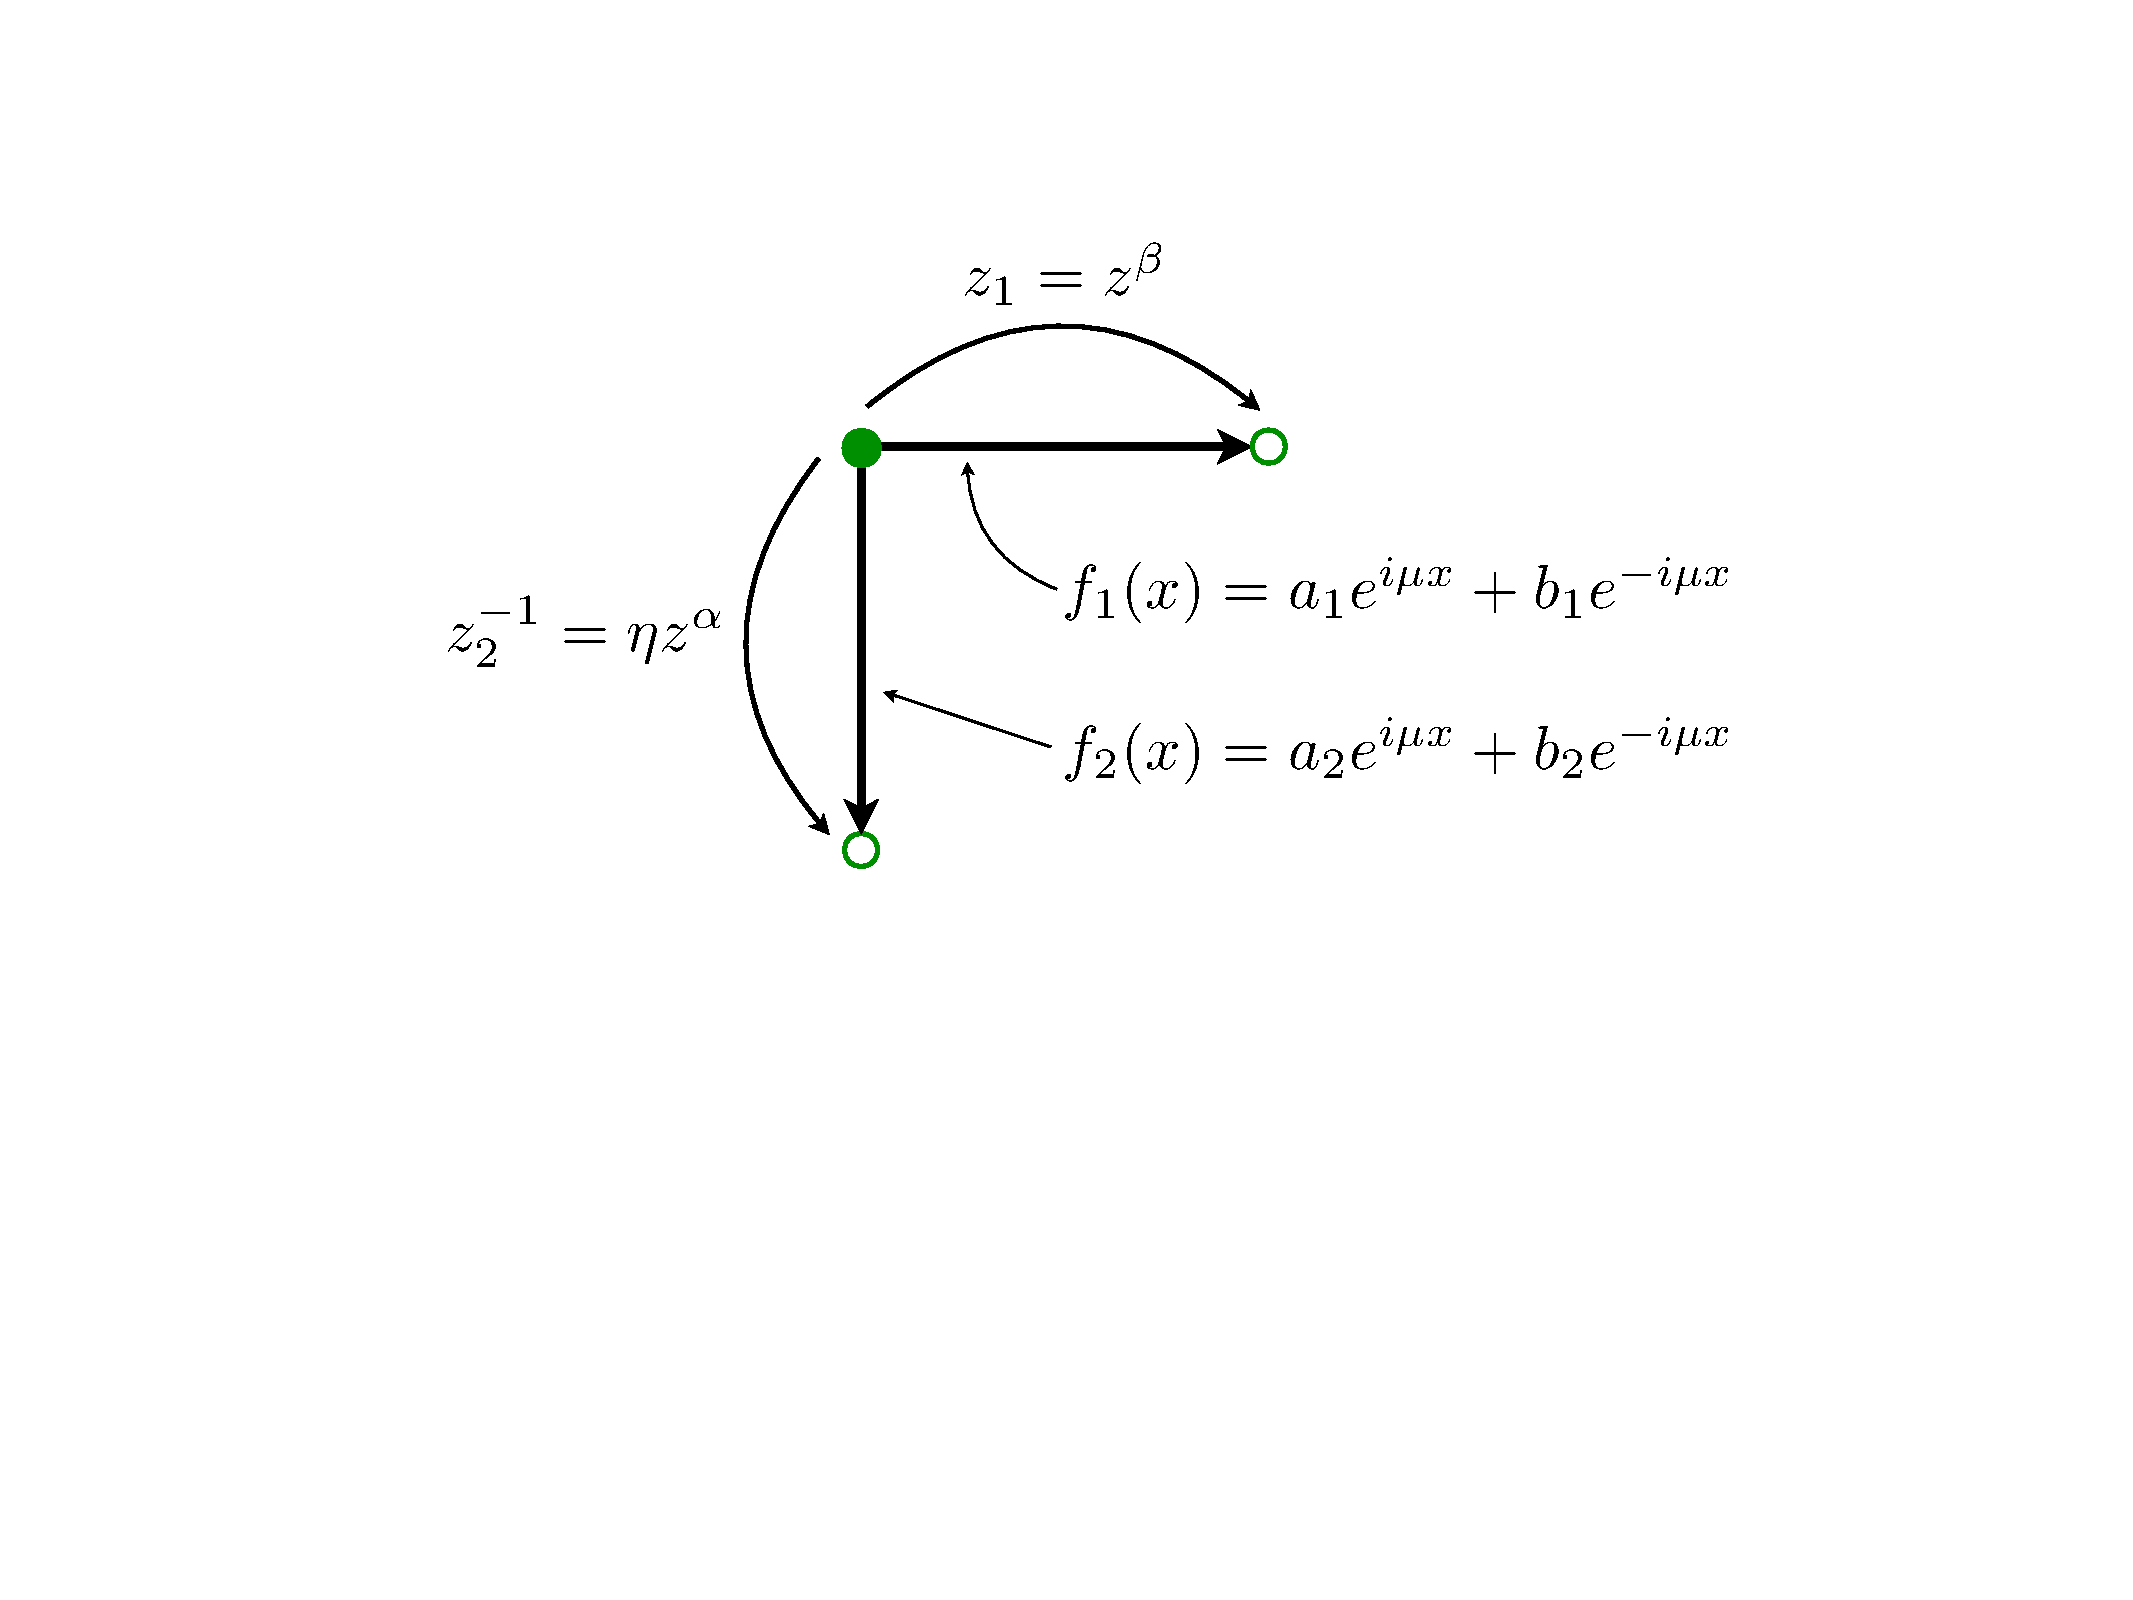
\includegraphics{FundamentalDomain.pdf}}}
\caption{\small A fundamental domain ...}
\label{fig:FundamentalDomain}
\end{figure}

The continuity and zero-flux conditions result in a homogeneous linear system for the coefficients $a_{1,2}$ and $b_{1,2}$.  After some reduction and with the notation $\zeta:=e^{i\mu}$ the system can be written as
%
\begin{equation}
\renewcommand{\arraystretch}{1.3}
\left[
  \begin{array}{cccc}
    1 & 1 & -1 & -1 \\
    z_1-\zeta & z_1\!-\!\zeta^{-1} & 0 & 0 \\
    0 & 0 & z_2^{-1}\!-\!\zeta & z_1^{-1}\!-\!\zeta^{-1} \\
    1\!-\!\zeta z_1^{-1} & 0 & 1\!-\!\zeta z_2 & 0
  \end{array}
\right]
\left[
  \begin{array}{c}
    a_1 \\ b_1 \\ a_2 \\ b_2
  \end{array}
\right]
=
\left[
  \begin{array}{c}
    0 \\ 0 \\ 0 \\ 0
  \end{array}
\right]
\end{equation}
%
The determinant of this matrix is
%
\begin{equation}
  D(z_1,z_2,\zeta) = (\zeta-\zeta^{-1}) \left[\, 2(\zeta+\zeta^{-1}) - \left( z_1+z_1^{-1} + z_2+z_2^{-1} \right) \right]
\end{equation}
%
and leads to the well-known dispersion relation
%
\begin{equation}
  z_1+z_1^{-1} + z_2+z_2^{-1} = 4\cos\mu
\end{equation}
%
whenever $\sin\mu\not=0$.

When the dispersion relation is satisfied, the coefficients are found to be
%
\begin{equation}\label{coefficients}
  \renewcommand{\arraystretch}{1.1}
\left[
  \begin{array}{c}
      a_1 \\ b_1 \\ a_2 \\ b_2
  \end{array}
\right]
=\,
c \left[
  \begin{array}{c}
      z_1-\zeta^{-1} \\ -z_1 + \zeta \\ z_2^{-1} - \zeta^{-1} \\ -z_2^{-1} + \zeta
  \end{array}
\right].
\end{equation}
%

Define the functions $g^\pm_{1,2}$ by
%
\begin{equation}
  g^\pm_{1,2}(x) := f_{1,2}(x) \pm i f'_{1,2}(x) = a_{1,2} (1\mp\mu) e^{i\mu x} + b_{1,2} (1\pm\mu) e^{-i\mu x}.
\end{equation}
%
With $c=1$ in (\ref{coefficients}), one obtains
%
\begin{eqnarray}
  g_1^\pm(x) &=& (1\mp\mu)\left( z_1e^{i\mu x} - e^{i\mu(x-1)} \right)
                             - (1\pm\mu)\left( z_1^{-i\mu x} - e^{-i\mu(x-1)} \right) \\
  g_2^\pm(x) &=& (1\mp\mu)\left( z_2^{-1}e^{i\mu x} - e^{i\mu(x-1)} \right)
                             - (1\pm\mu)\left( z_2^{-1}e^{-i\mu x} - e^{-i\mu(x-1)} \right)                             
\end{eqnarray}
%



\subsection{Lattice tubes}


(Refer to \cite{KuchmentPost2007} ...) ... write two positive integers whose $\gcd$ is $\delta$ as $\alpha\delta$ and $\beta\delta$, with $\gcd(\alpha,\beta)=1$ ...

Fig.\,\ref{fig:Tube} illustrates how the quantum graph sheet $\Gamma$ is rolled into a tube $T$ by identifying points that differ by an integer multiple of a given integer vector $( \delta\alpha, \delta\beta )$.   It is assumed that $\gcd(\alpha,\beta)=1$ and $\alpha<\beta$.
In other words, let $\Lambda$ be the one-dimensional subgroup of $\ZZ^2$ generated by $( \delta\alpha, \delta\beta )$.  This group acts by skew translation on $\Gamma$, and $T$ is the quotient space: $T=\Gamma/\Lambda$.
An general element of $T$ is an equivalence class $\langle v \rangle = \left\{ v + \ell w : w\in\Lambda \right\}$, where $v\in\ZZ^2$.
A convenient fundamental domain for $T$, denoted by $\tilde T$, is depicted in Fig.~\ref{fig:Tube} by the solid green part of $\Gamma$ in the case that $\delta=1$.

The $\ZZ^2$ action in $\Gamma$ induces an action on $T$ by $g\langle v \rangle = \langle g\,v \rangle$ for $v\in\Gamma$ and $g\in\ZZ^2$.  The kernel of the action is $\Lambda$, and thus can be reduced to a faithful action by the quotient group $\ZZ^2/\Lambda$.  A subgroup of $\ZZ^2/\Lambda$, isomorphic to $\ZZ$, is inherited from the horizontal translations of~$\Gamma$.  Its action is represented in Fig.\,\ref{fig:Tube} by horizontal translations of the fundamental domain~$\tilde T$.  More precisely, $\ZZ$ acts on $T$ as the image of the injection
%
\begin{equation}
\renewcommand{\arraystretch}{1.1}
\left.
\begin{array}{ccccc}
  \ZZ &\to& \ZZ^2 &\to& \ZZ/\Lambda  \\
  g &\mapsto& (g,0) &\mapsto& \langle (g,0) \rangle .
\end{array}
\right.
\end{equation}
%
The group $\ZZ$, together with this action on $T$ will be referred to as the {\itshape h-translation group} for~$T$.  (This term preserves the fact that the action is inherited from horizontal translations of $\Gamma$, while avoiding the term ``horizontal translation group", which is not suitable for the 1-periodic structure $T$.)  In short, the h-translation by $g\in\ZZ$ is given by
%
\begin{equation}
  g \langle (m,n) \rangle \,=\, \langle (m+g,n) \rangle
 \qquad
 \text{(h-translations of $T$)}.
\end{equation}
%

A fundamental domain in $T$ for the h-translation group $\ZZ$ is depicted in Fig.~\ref{fig:Tube} in blue and denoted by $W$.  It is obtained by first drawing a path of horizontal and vertical line segments in $\Gamma$, connecting vertices in such a way that each segment intersects the (black)~line
%
\begin{equation}
  L = \left\{ (x,y): \alpha y - \beta x = 0 \right\}  
\end{equation}
%
in the $(x,y)$-plane $\RR^2$ exactly once \notesps{and ...}; and then adding horizontal pendant edges emanating leftward from all vertices in the interiors of the vertical line segments.  Each horizontal line segment consists of exactly one edge, and there are exactly $\delta(\beta-\alpha)$ pendant horizontal edges emanating from the vertical line segments.

The Floquet modes of the tube $T=\Gamma/\Lambda$ are obtained from those of $\Gamma$ by retaining those that are invariant under the skew translation group $\Lambda$.  This means that, besides satisfying the dispersion relation for $\Gamma$, the vector $(z_1,z_2)$ of Floquet multipliers must produce a multiplier of $1$ for the translation vector $\langle \delta\alpha,\delta\beta \rangle$:



\begin{figure}  %%%%%%%%%%%%%%%%% FIGURE %%%%%%%%%%%%%%%%%%
\centerline{\scalebox{0.5}{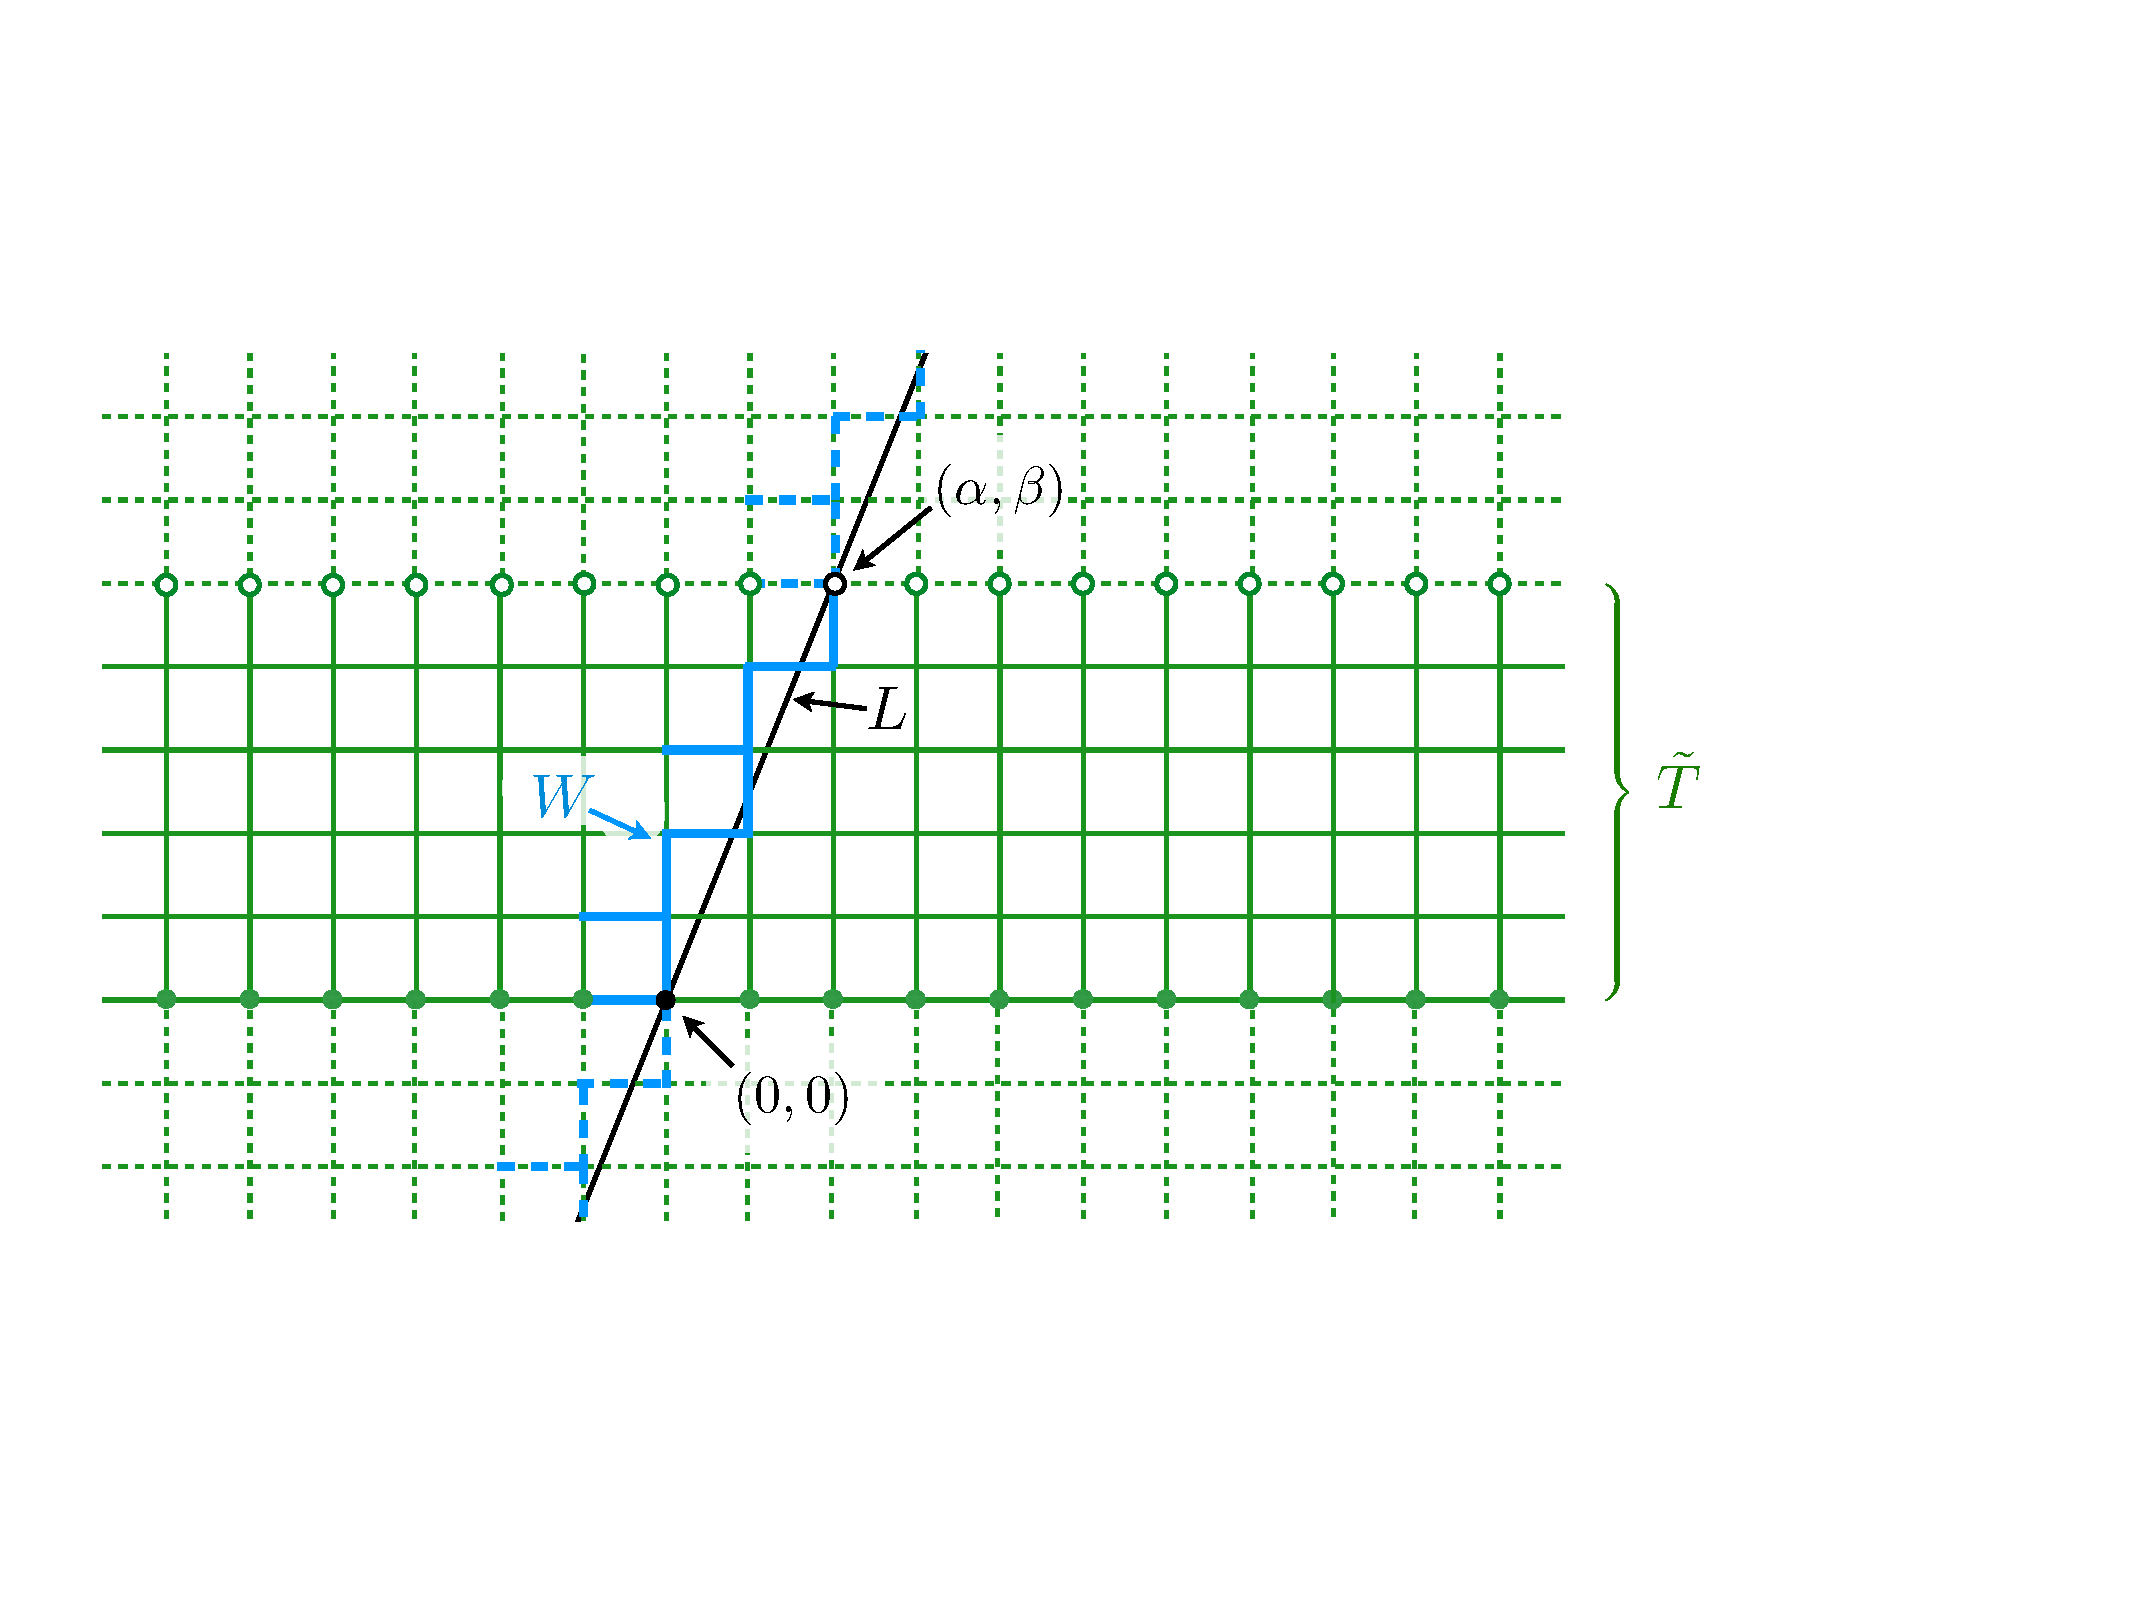
\includegraphics{Tube1.pdf}}}
\caption{\small Forming a tube and a fundamental domain $W$ (in blue) for shifts of the tube ...}
\label{fig:Tube}
\end{figure}



%
\begin{equation}\label{zequation1}
  \renewcommand{\arraystretch}{1.1}
\left\{
  \begin{array}{l}
    z_1 + z_1^{-1} + z_2 + z_2^{-1} = 4\cos\mu \\
    z_1^{\alpha\delta} z_2^{\beta\delta} = 1.
  \end{array}
\right.
\end{equation}
%

The condition $z_1^{\alpha\delta} z_2^{\beta\delta} = 1$ is equivalent to 
%
\begin{equation}
  z_1^\alpha z_2^\beta = \cchi{\frac{\ell}{\delta}}
  \quad \text{for some integer } \ell:\,0\leq\ell<\delta,
\end{equation}
%
in which $\chi(t) = e^{2\pi it}$.  Thus (\ref{zequation1}) is equivalent to the existence of $\ell:\,0\leq\ell<\delta$ such that
%
\begin{equation}\label{zequation2}
  \renewcommand{\arraystretch}{1.1}
\left\{
  \begin{array}{l}
    z_1 + z_1^{-1} + z_2 + z_2^{-1} = 4\cos\mu \\
    z_1^\alpha z_2^\beta = \chi\!\left( \frac{\ell}{\delta} \right). \\
  \end{array}
\right.
\end{equation}
%

The following lemma characterizes the solutions of (\ref{zequation2}).

\begin{lemma}\label{lemma:zequation}
If $\alpha$ and $\beta$ are positive integers with $\gcd(\alpha,\beta)=1$ and $(z_1,z_2)\in(\CC^*)^2$, then (\ref{zequation2}) holds if and only if there exists $z\in\CC^*$ such that
%
\begin{equation}\label{zequation3}
  \renewcommand{\arraystretch}{1.1}
\left\{
  \begin{array}{l}
    z^\beta + z^{-\beta} + \eta z^\alpha + \eta^{-1} z^{-\alpha} = 4\cos\mu\,,\; \text{ with } \eta=\cchi{\frac{-\ell}{\beta\delta}} \\
    z_1 = z^{\beta} \\
    z_2 = \eta^{-1} z^{-\alpha}\,.
  \end{array}
\right.
\end{equation}
%
Such $z$ is unique.  The same pair $(z_1,z_2)$ satisfies the modification of the system (\ref{zequation3}) by the replacements
%
\begin{eqnarray}
  z \mapsto \cchi{\frac{j}{\beta}}z,
  \quad
  \eta \mapsto \cchi{\frac{-j\alpha}{\beta}}\eta,
\end{eqnarray}
%
featuring the isomorphism $\cchi{\frac{j}{\beta}}\mapsto\cchi{\frac{-j\alpha}{\beta}}$ of the group of $\beta^\text{th}$ roots of $1$.

If $z$ satisfies the first equation in the system (\ref{zequation3}) and $|z|\not=1$, then $z$ is a simple root of the equation.
\end{lemma}

\begin{proof}
To prove that (\ref{zequation3}) implies (\ref{zequation2}) is straightforward.
  To prove the uniqueness of the number $z\in\CC^*$ that satisfies (\ref{zequation3}), suppose $\eta^{-1}z^{-\alpha}=\eta^{-1}w^{-\alpha}$ and $z^\beta=w^\beta$ for some $z$ and $w$ in $\CC^*$.  Then $(zw^{-1})^\alpha=1=(zw^{-1})^\beta$.  Since $\gcd(\alpha,\beta)=1$, $zw^{-1}=1$, so that $z=w$.
  
  To prove the existence of such $z$ under the assumption of (\ref{zequation2}), suppose that $z_1^\alpha z_2^\beta=\zeta:=\cchi{\frac{\ell}{\delta}}$, and let $\eta$ be such that $\eta^{-\beta}=\zeta$.  Then choosing numbers $w_1$ and $w_2$ such that $z_1=w_1^\beta$ and $z_2=\eta^{-1}w_2^{-\alpha}$ yields $(w_1w_2^{-1})^{\alpha\beta}=1$ and therefore $w_1w_2^{-1}=\cchi{\frac{r}{\alpha\beta}}$ for some integer $r$.  Since $\gcd(\alpha,\beta)=1$, there exist integers $m$ and $n$ such that $r=-m\alpha + n\beta$, or
%
\begin{equation}
  \frac{r}{\alpha\beta} = -\frac{m}{\beta} + \frac{n}{\alpha}\,.
\end{equation}
%
This implies that
%
\begin{equation}
  w_1w_2^{-1} = \cchi{\frac{-m}{\beta}} \cchi{\frac{n}{\alpha}},
\end{equation}
%
so that $w_1\cchi{\frac{m}{\beta}}=w_2\cchi{\frac{n}{\alpha}}:=z$.  This is the desired number since
$z^\beta=w_1^\beta=z_1$ and $\eta^{-1}z^{-\alpha}=\eta^{-1}w_2^{-\alpha} = z_2$ and first equation of (\ref{zequation2}) becomes the first equation of (\ref{zequation3}).

The condition for a root $z$ of the Laurent polynomial in (\ref{zequation3}) to be a multiple root is
%
\begin{equation}\label{multipleroot}
  \beta\left( z^\beta - z^{-\beta} \right) = -\alpha\left( \eta z^\alpha - \eta^{-1} z^{-\alpha} \right).
\end{equation}
%
Both sides of this equation lie on ellipses in $\CC$ with vertical major axis.
The left side lies on an ellipse with major radius $\beta\left( |z|^\beta + |z|^{-\beta} \right)$ and minor radius $\beta\left| |z|^\beta - |z|^{-\beta} \right|$, and the right side lies on an ellipse with major radius $\alpha\left( |z|^\alpha + |z|^{-\alpha} \right)$ and minor radius $\alpha\big| |z|^\alpha - |z|^{-\alpha} \big|$.  The assumptions $\beta>\alpha$ and $|z|\not=1$ imply
$\beta\left( |z|^\beta + |z|^{-\beta} \right)>\alpha\left( |z|^\alpha + |z|^{-\alpha} \right)$
and $\beta\big| |z|^\beta - |z|^{-\beta} \big|>\alpha\big| |z|^\alpha - |z|^{-\alpha} \big|$,
so that the two ellipses do not intersect.  Thus (\ref{multipleroot}) cannot hold and $z$ is therefore a simple~root.
\end{proof}



\begin{theorem}\label{thm:zequation}
If $\alpha$ and $\beta$ are positive integers with $\gcd(\alpha,\beta)=1$ and $\delta$ is a positive integer, then
the set of solutions $(z_1,z_2)\in(\CC^*)^2$ to the system (\ref{zequation1}) is the {\em disjoint} union
%
\begin{equation}
  \bigcup\limits_{\ell=0}^{\delta-1} {\mathcal Z}_\ell
\end{equation}
%
of the solutions sets of (\ref{zequation2}),
%
\begin{equation}\label{union}
  {\mathcal Z}_\ell \,=\,
  \left\{ (z^\beta, \eta^{-1}z^{-\alpha})\,:\,
    z^\beta + z^{-\beta} + \eta z^\alpha + \eta^{-1} z^{-\alpha} = 4\cos\mu,\; z\in\CC^*,\; \eta=\cchi{\frac{-\ell}{\beta\delta}}
  \right\}.
\end{equation}
%
\end{theorem}

\begin{proof}
Because the system (\ref{zequation1}) is equivalent to the existence of an integer $\ell:0\leq\ell<\delta$ such that (\ref{zequation2}) holds, Lemma~\ref{lemma:zequation} establishes the union (\ref{union}).  To prove that it is disjoint, suppose that
%
\begin{equation}
  \renewcommand{\arraystretch}{1.1}
\left.
  \begin{array}{r}
    z_1=z^{\beta} = w^{\beta} \\
    z_2 = \eta^{-1} z^{-\alpha} = \nu^{-1} w^{-\alpha}
  \end{array}
\right\}
\quad\text{with $\eta=\cchi{\frac{-\ell}{\beta\delta}}$ and $\nu=\cchi{\frac{-k}{\beta\delta}}$}
\end{equation}
%
and $0\leq\ell<\delta$ and $0\leq k<\delta$.
One has $\eta\nu^{-1}=(wz^{-1})^\alpha$ and $(wz^{-1})^\beta=1$, so that
$(\eta\nu^{-1})^\beta = (wz^{-1})^{\alpha\beta} = 1^\alpha = 1$, and therefore $\cchi{\frac{k-\ell}{\delta}}=1$.  Since $|k-\ell|<\delta$, one has $\left| \frac{k-\ell}{\delta} \right|<1$, which together with $\cchi{\frac{k-\ell}{\delta}}=1$ yields $\frac{k-\ell}{\delta}=0$ and hence $\eta=\nu$.
\end{proof}


%%%%%%%%%%%%%%%%%%%% THEOREM %%%%%%%%%%%%%%%%%%%%
\begin{theorem}\label{thm:modes} Let $\lambda\in\CC\setminus\sigma_D$, and let $\mu^2=\lambda$.

(a)  Let $g\in\ZZ$ be given, and let $u\in H^2_*(gW)$ satisfy $Hu=\lambda u$ (at internal vertices, the only assumption on $u$ is continuity).  Then $u$ has a unique extension $\tilde u \in \Hloc(T)$ to the full tube such that $H\tilde u=\lambda \tilde u$ (\,$\tilde u$ satisfies the standard condition at each vertex).

(b)  A basis of the space $\left\{ u\in\Hloc(T) \,:\, Hu = \lambda u \right\}$ consists of the $2\beta$ Floquet modes ...
\end{theorem}

\begin{proof}
  Part (a) ... gotta just look at it yourself.
  
  Part (a) of the theorem shows that the dimension of the space $\left\{ u\in\Hloc(T) \,:\, Hu = \lambda u \right\}$ is equal to the dimension of the space
%
\begin{equation}
  \left\{ u\in\Hstar(W) \,:\, Hu=\lambda u \right\}.
\end{equation}
%
The graph $W$ has $2\beta$ edges; let edge $e$ be parameterized by $x_e\in(0,1)$ from top to bottom or from right to left.  The equation $Hu=\lambda u$ implies that, on each edge,
%
\begin{equation}
  u(x_e) = a_e \cos \mu x_e + b_e\, \mu^{-1} \sin \mu x_e\,
\end{equation}
%
for some numbers $a_e$ and $b_e$.  Continuity at the vertices implies $2\beta$ linear conditions among the $4\beta$ numbers $\{a_e,b_e\}_{e\in E(\Gamma)}$.  The rank of the matrix for these linear relations is $2\beta$:  If the edges are ordered by first traversing the unique cycle in $W$ and then including the pendant edges, the matrix is has an upper-left block that is block-cyclic and a lower-right block that is block-diagonal, with the minor blocks being $1\!\times\!2$ matrices.
As an illustration with $(\alpha,\beta)=(2,5)$, as in Fig.~\ref{fig:Tube}, the matrix is
%
\begin{equation}
  \renewcommand{\arraystretch}{1.1}
\left[
\begin{array}{cccccccccccccc|cccccc}
  c&s&1&0&&&&&&&&&&&&&&&& \\
  &&c&s&1&0&&&&&&&&&&&&&& \\
  &&&&c&s&1&0&&&&&&&&&&&& \\
  &&&&&&c&s&1&0&&&&&&&&&& \\
  &&&&&&&&c&s&1&0&&&&&&&& \\
  &&&&&&&&&&c&s&1&0&&&&&& \\
  1&0&&&&&&&&&&&c&s&&&&&& \\
  \hline
   &&&&&&1&0&&&&&&&-1&0&&&& \\
   &&&&&&&&&&&&1&0&&&-1&0&& \\
   1&0&&&&&&&&&&&&&&&&&-1&0   
\end{array}
\right],
\end{equation}
%
in which \,$c=-\cos\mu$\, and \,$s=-\mu^{-1}\sin\mu$.
That the rows of this matrix are linearly independent can be easily checked.

Thus the space $\left\{ u\in\Hloc(T) \,:\, Hu = \lambda u \right\}$ is $2\beta$-dimensional.  To prove that the $2\beta$ Floquet modes form a basis, it is sufficient to prove that the vectors containing the values of the modes at $2\beta$ points of $T$ are linearly independent.  Given $p\in T$ at which none of the Floquet modes vanish, consider the column vectors obtained by evaluating the Floquet modes at the $2\beta$ points $g\!\cdot\! p$, for $g=0,\dots,2\beta-1$.  In the generic case that all roots are distinct, the square matrix formed by these column vectors has the form
%
\begin{equation}
  \renewcommand{\arraystretch}{1.1}
\left[
\begin{array}{lllll}
  c_1 & c_2 & c_3 & \cdots & c_{2\beta} \\
  c_1z_1 & c_2z_2 & c_3z_3 & \cdots & c_{2\beta}z_{2\beta} \\
  c_1z_1^2 & c_2z_2^2 & c_3z_3^2 & \cdots & c_{2\beta}z_{2\beta}^2 \\
  \vdots & \vdots & \vdots & \vdots & \vdots \\
  c_1z_1^{2\beta-1} & c_2z_2^{2\beta-1} & c_3z_3^{2\beta-1} & \cdots & c_{2\beta}z_{2\beta}^{2\beta-1}
\end{array}
\right]
\end{equation}
%
with all $c_i$ nonzero.  By dividing the $j^\text{th}$ column by $c_j$, one obtains a Vandermonde matrix, which is nonsingular.  In the general case, in which some roots may be multiple, one obtains a generalized Vandermonde matrix \cite{Sobczyk2002}, which is nonsingular.
\end{proof}


\section{The half-infinite tube}\label{sec:HalfTube} %%%%%%%%%%%%%%%%%%%%%%

Ideas to elaborate:

\begin{itemize}
\item Cutting the tube along the vector $(\alpha\delta,\beta\delta)$ to obtain the graph $T_+$.

\item Start with $\alpha+\beta$ free vertices (one of them is split into two).

\item Maximal operator $H_+$, with domain $\Dmax$ (no boundary-vertex conditions) and minimal operator $H_-$ with domain $\Dmin$ (zero value and derivative at each boundary vertex).  $H_+$ and $H_-$ are adjoints of one another, and we consider self-adjoint extensions of $H_-$, which are contained in $H_+$.

\item Description of all self-adjoint extensions of $H_-$.  Each is given by $\alpha+\beta$ linear conditions on the boundary data at the free vertices.

\item {\em Auxiliary boundary fields} in $\Dmax$, which have support on one of the $\alpha$ red backward-L-shaped domains (boundary ---a pair of pendant edges joined by a vertex), vanish on the red vertex, and have zero ``flux".  For a given frequency, there are $\alpha$ independent auxiliary boundary fields, one for each boundary frill.

\item Theorem: Given a frequency $\lambda$ (or $\mu$), if a field is known on one translate of $W$ contained completely in $T_+$, then the field is determined up to a combination of the $\alpha$ auxiliary boundary fields for $\lambda$.

\item Reflection off of the boundary of the tube, for fixed frequency $\lambda$ and fixed self-adjoint extension.  Given: $\beta$ coefficients of incoming Floquet modes.  Solve for:  $\beta$ coefficients of outgoing Floquet modes and $\alpha$ coefficients of the auxiliary boundary fields, subject to the $\alpha+\beta$ conditions defining the self-adjoint operator.

\item Bound states:  Set all incoming modes coefficients to zero, and seek frequencies (and self-adjoint extensions) for which the algebraic system for the reflection problem has nontrivial solutions.

\item Do specific self-adjoint operators (full picture too complex?):  Free vertices (Neumann); pinned vertices (Dirichlet); joined vertices with continuity and zero flux.  Hopefully these can be completely analyzed.

\end{itemize}


\subsection{Forming the half-tube}\label{sec:cutting}  %%%%%%%%%%%%%%%%

... cut the graph $\Gamma$ along the line $L=\left\{ (x,y): \alpha y - \beta x = 0 \right\}$.  The points of intersection between $\Gamma$ and $L$, marked with black dots or circles in Fig.~\ref{fig:HalfTube} (left), are
%
\begin{equation}
  \renewcommand{\arraystretch}{1.1}
\left.
\begin{array}{ll}
  v^1_j = \big( j,\frac{\beta j}{\alpha} \big) & \text{(intersections of $L$ with vertical edges)} \\
  v^2_j = \big( \frac{\alpha j}{\beta}, j \big) & \text{(intersections of $L$ with horizontal edges)}
\end{array}
\right.
(j\in\ZZ).
\end{equation}
%
The intersection of the sets $\left\{ v^1_j : j\in\ZZ \right\}$ and $\left\{ v^2_j : j\in\ZZ \right\}$ is the set of vertices of $\Gamma$ that intersect $L$, which is just the integer multiples of the point $(\alpha,\beta)$, as illustrated in Fig.~\ref{fig:HalfTube}.

When forming the tube $T = \Gamma/\Lambda$, the points $v^1_j$ are placed into $\delta\alpha$ equivalence classes $\langle v^1_j \rangle$, 
and the points $v^2_j$ are placed into $\delta\beta$ equivalence classes $\langle v^2_j \rangle$,
%
\begin{equation}
\renewcommand{\arraystretch}{1.1}
\left.
\begin{array}{l}
    \langle v^1_j \rangle = \{ v^1_j + \ell (\delta\alpha,\delta\beta):\ell\in\ZZ\} \\
      %& j=0,\dots, \delta\alpha-1, \\
    \langle v^2_j \rangle = \{ v^2_j + \ell (\delta\alpha,\delta\beta):\ell\in\ZZ\}.
      %& j=0,\dots, \delta\beta-1.
\end{array}
\right.
\end{equation}
%
These equivalence classes are points on the tube $T$.

Each equivalence class is represented by an element of one of the sets
%
\begin{equation}
  \left\{ v^1_j \right\}_{j=0}^{\delta\alpha-1}
  \qquad \text{and} \qquad
  \left\{ v^2_j \right\}_{j=0}^{\delta\beta-1}\,.
\end{equation}
%
The union of these two sets is indicated by solid black dots in Fig.~\ref{fig:HalfTube} (left) for $(\alpha,\beta)=(2,5)$.
These sets are not disjoint but intersect at the $\delta$ points $\left\{ \ell(\alpha,\beta) \right\}_{\ell=0}^{\delta-1}$, whose equivalence classes are vertices of $T$,
%
\begin{equation}
  \langle \ell(\alpha,\beta) \rangle
  = \langle v^1_{\alpha\ell} \rangle
  = \langle v^2_{\beta\ell} \rangle.
\end{equation}
%
The equivalence classes of the other points $v^1_j$ and $v^2_j$ lie in the interior of some edge of $T$.

Let us retain only the semi-infinite part of $T$ lying to the right of the cut along $L/\Lambda$ and place boundary vertices at the points $\left\{ \langle v^1_j \rangle, \langle v^2_j \rangle \right\}$ at which an edge was cut at an interior point.  Each point of the form $\left\{ \langle \ell(\alpha,\beta) \rangle \right\}_{\ell=0}^{\delta-1}$, which is already a vertex of $T$, has two edges emanating from it into the right semi-infinite part of $T$.  Each of these edges will receive one copy of the vertex; that is, the vertex is split into two boundary vertices, each adjacent to a single edge.  The resulting metric graph will be denoted by $T_+$.  Its $\delta(\alpha+\beta)$ boundary vertices (its set of leaves) are identified with the disjoint union
%
\begin{equation}
  \left\{ \langle v^1_j \rangle \right\}_{j=0}^{\delta\alpha-1}
   \mathring{\cup}
  \left\{ \langle v^2_j \rangle \right\}_{j=0}^{\delta\beta-1}.
%  \qquad
%  \text{(boundary vertices of $T_+$)}.
\end{equation}
%
Let the boundary vertex associated with $\langle v^1_j \rangle$ be denoted by $\tilde v^1_j$, with $\tilde v^1_{j+\delta\alpha}=\tilde v^1_j$.  Similarly, let the boundary vertex associated with $\langle v^2_j \rangle$ be denoted by $\tilde v^2_j$.  Thus the set of boundary vertices is the disjoint union
%
\begin{equation}
  \left\{ \tilde v^1_j \right\}_{j=0}^{\delta\alpha-1}
  \cup
  \left\{ \tilde v^2_j \right\}_{j=0}^{\delta\beta-1}\,
   \qquad
    \text{(boundary vertices of $T_+$)}.
\end{equation}
%
\notesps{Can this be explained more simply in terms of pendant edges instead of vertices?}

In the case that $\delta=1$, the boundary vertices can be represented on $\Gamma$ by the vertices $\left\{ v^1_j \right\}_{j=1}^\alpha$ and $\left\{ v^2_j \right\}_{j=0}^{\beta-1}$, as illustrated by the solid black dots in Fig.~\ref{fig:HalfTube} (right)---the vertices at $(0,0)=v^1_0=v^2_0$ and $(\alpha,\beta)=v^1_\alpha=v^2_\beta$, which were identified as one vertex in $T$ are distinct boundary vertices of $T_+$.




\begin{figure}  %%%%%%%%%%%%%%%%% FIGURE %%%%%%%%%%%%%%%%%%
\scalebox{0.47}{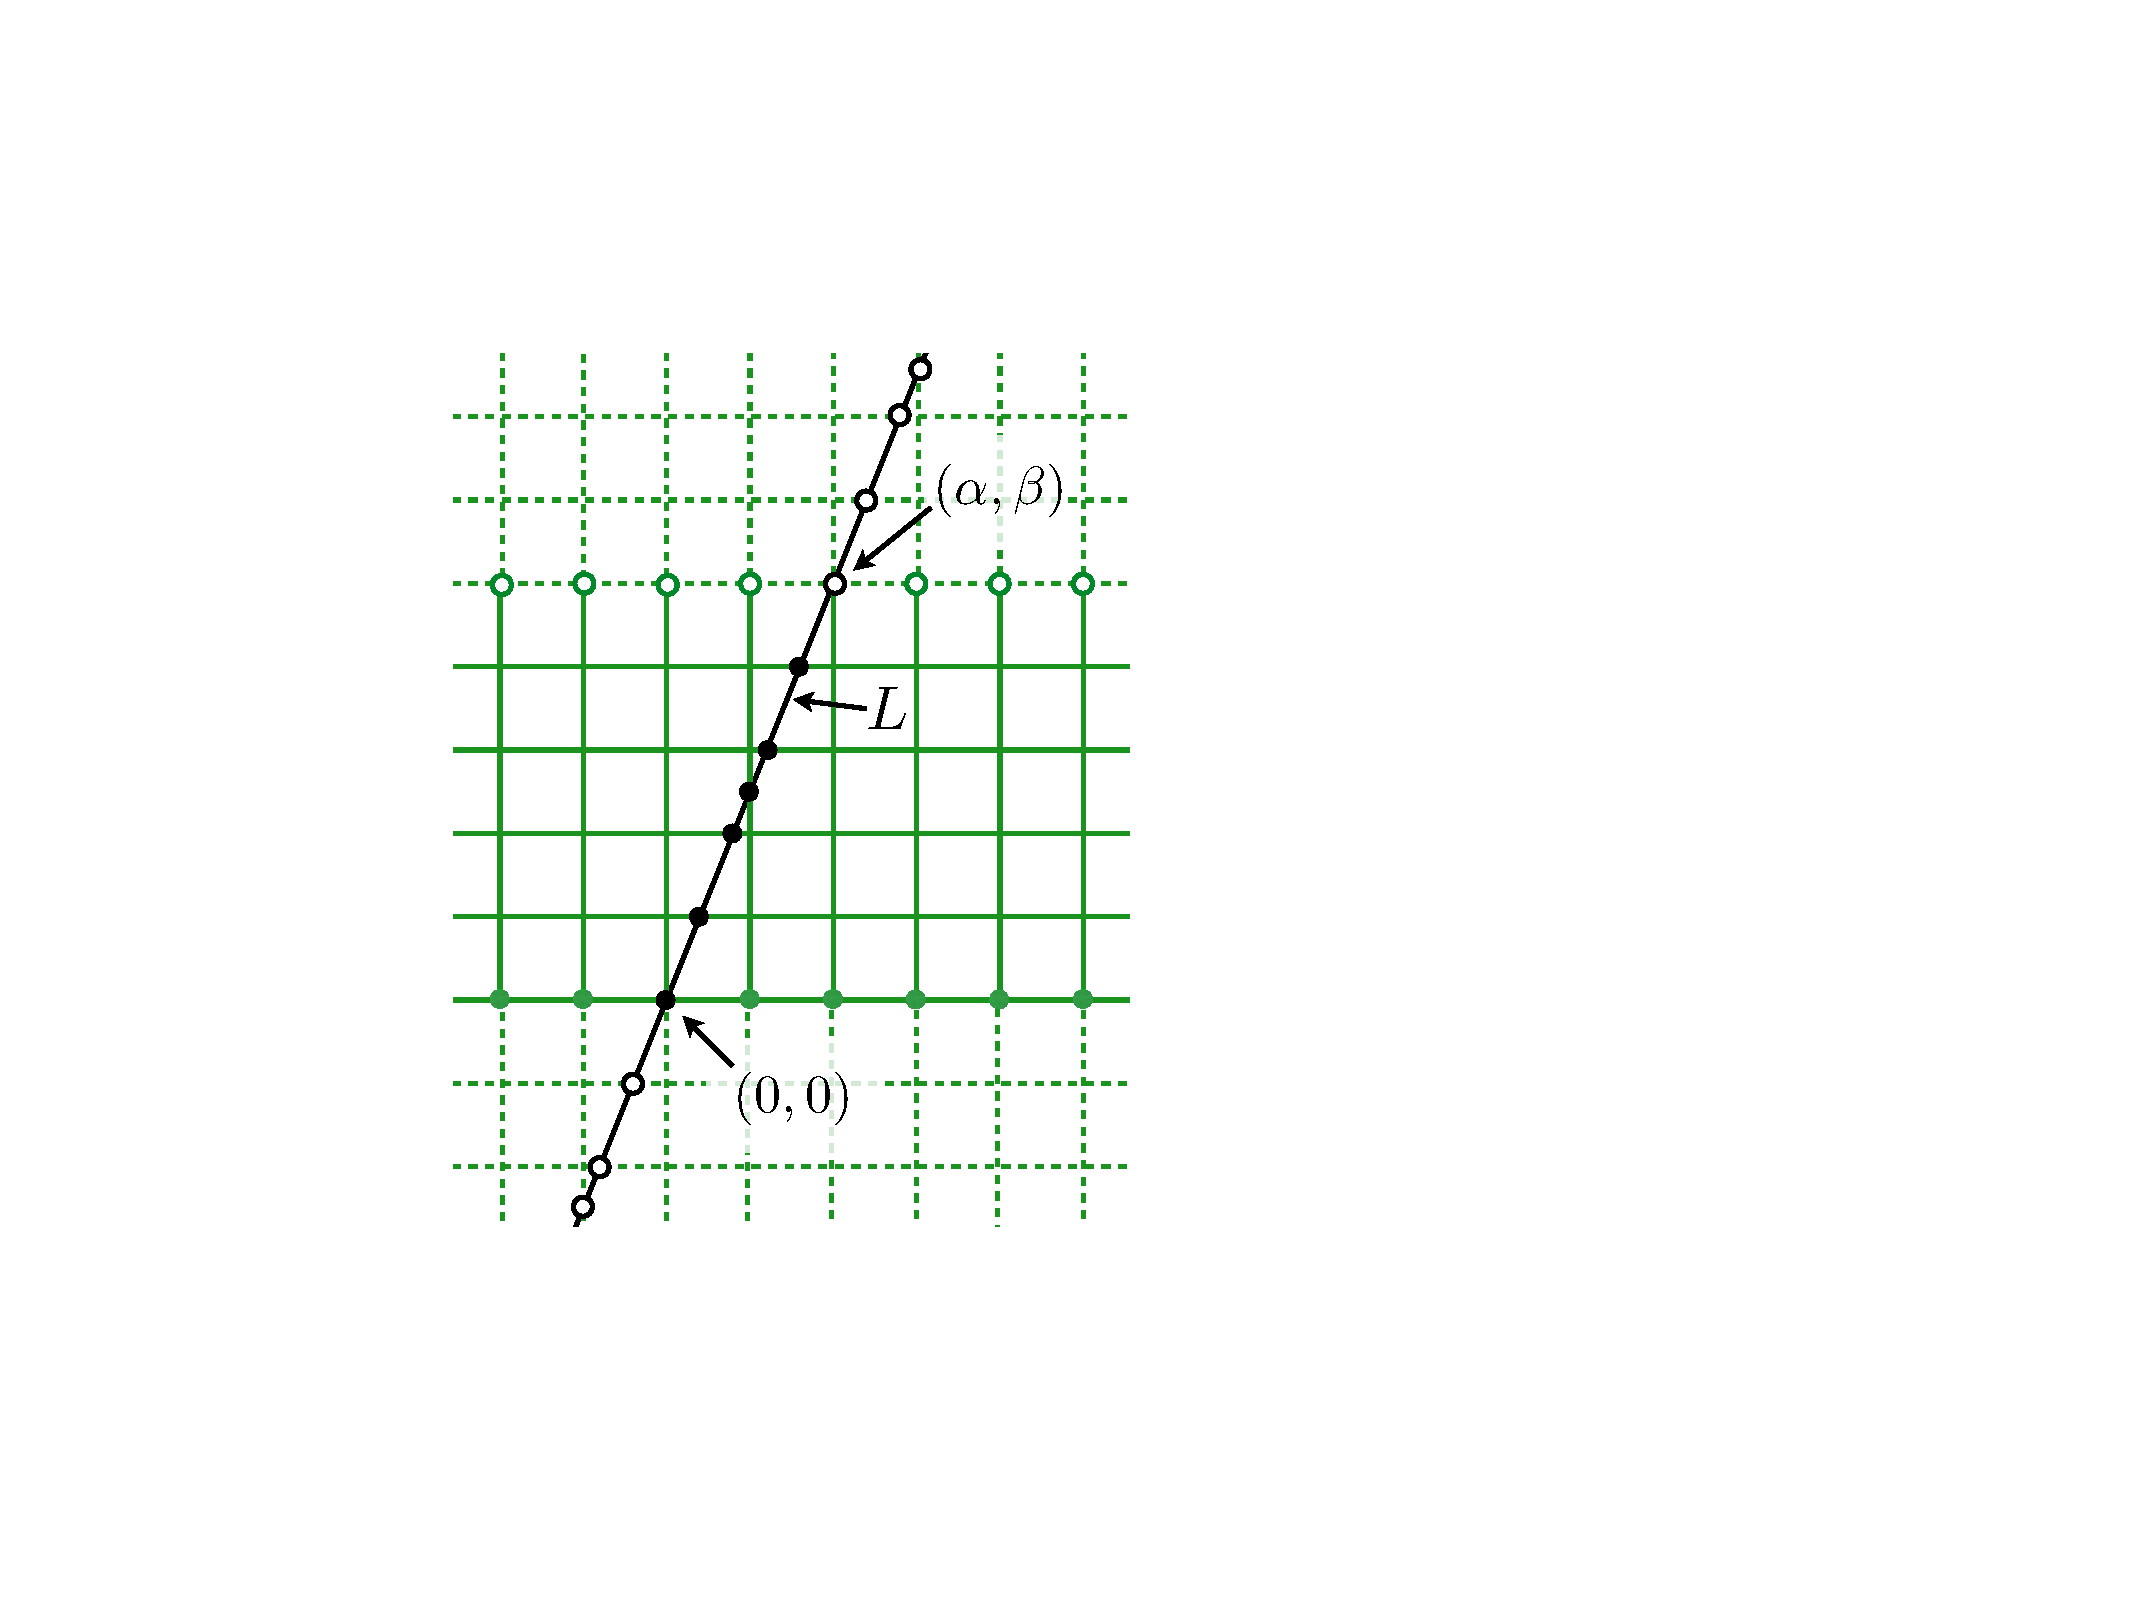
\includegraphics{Tube1b.pdf}}
\hfill
\scalebox{0.47}{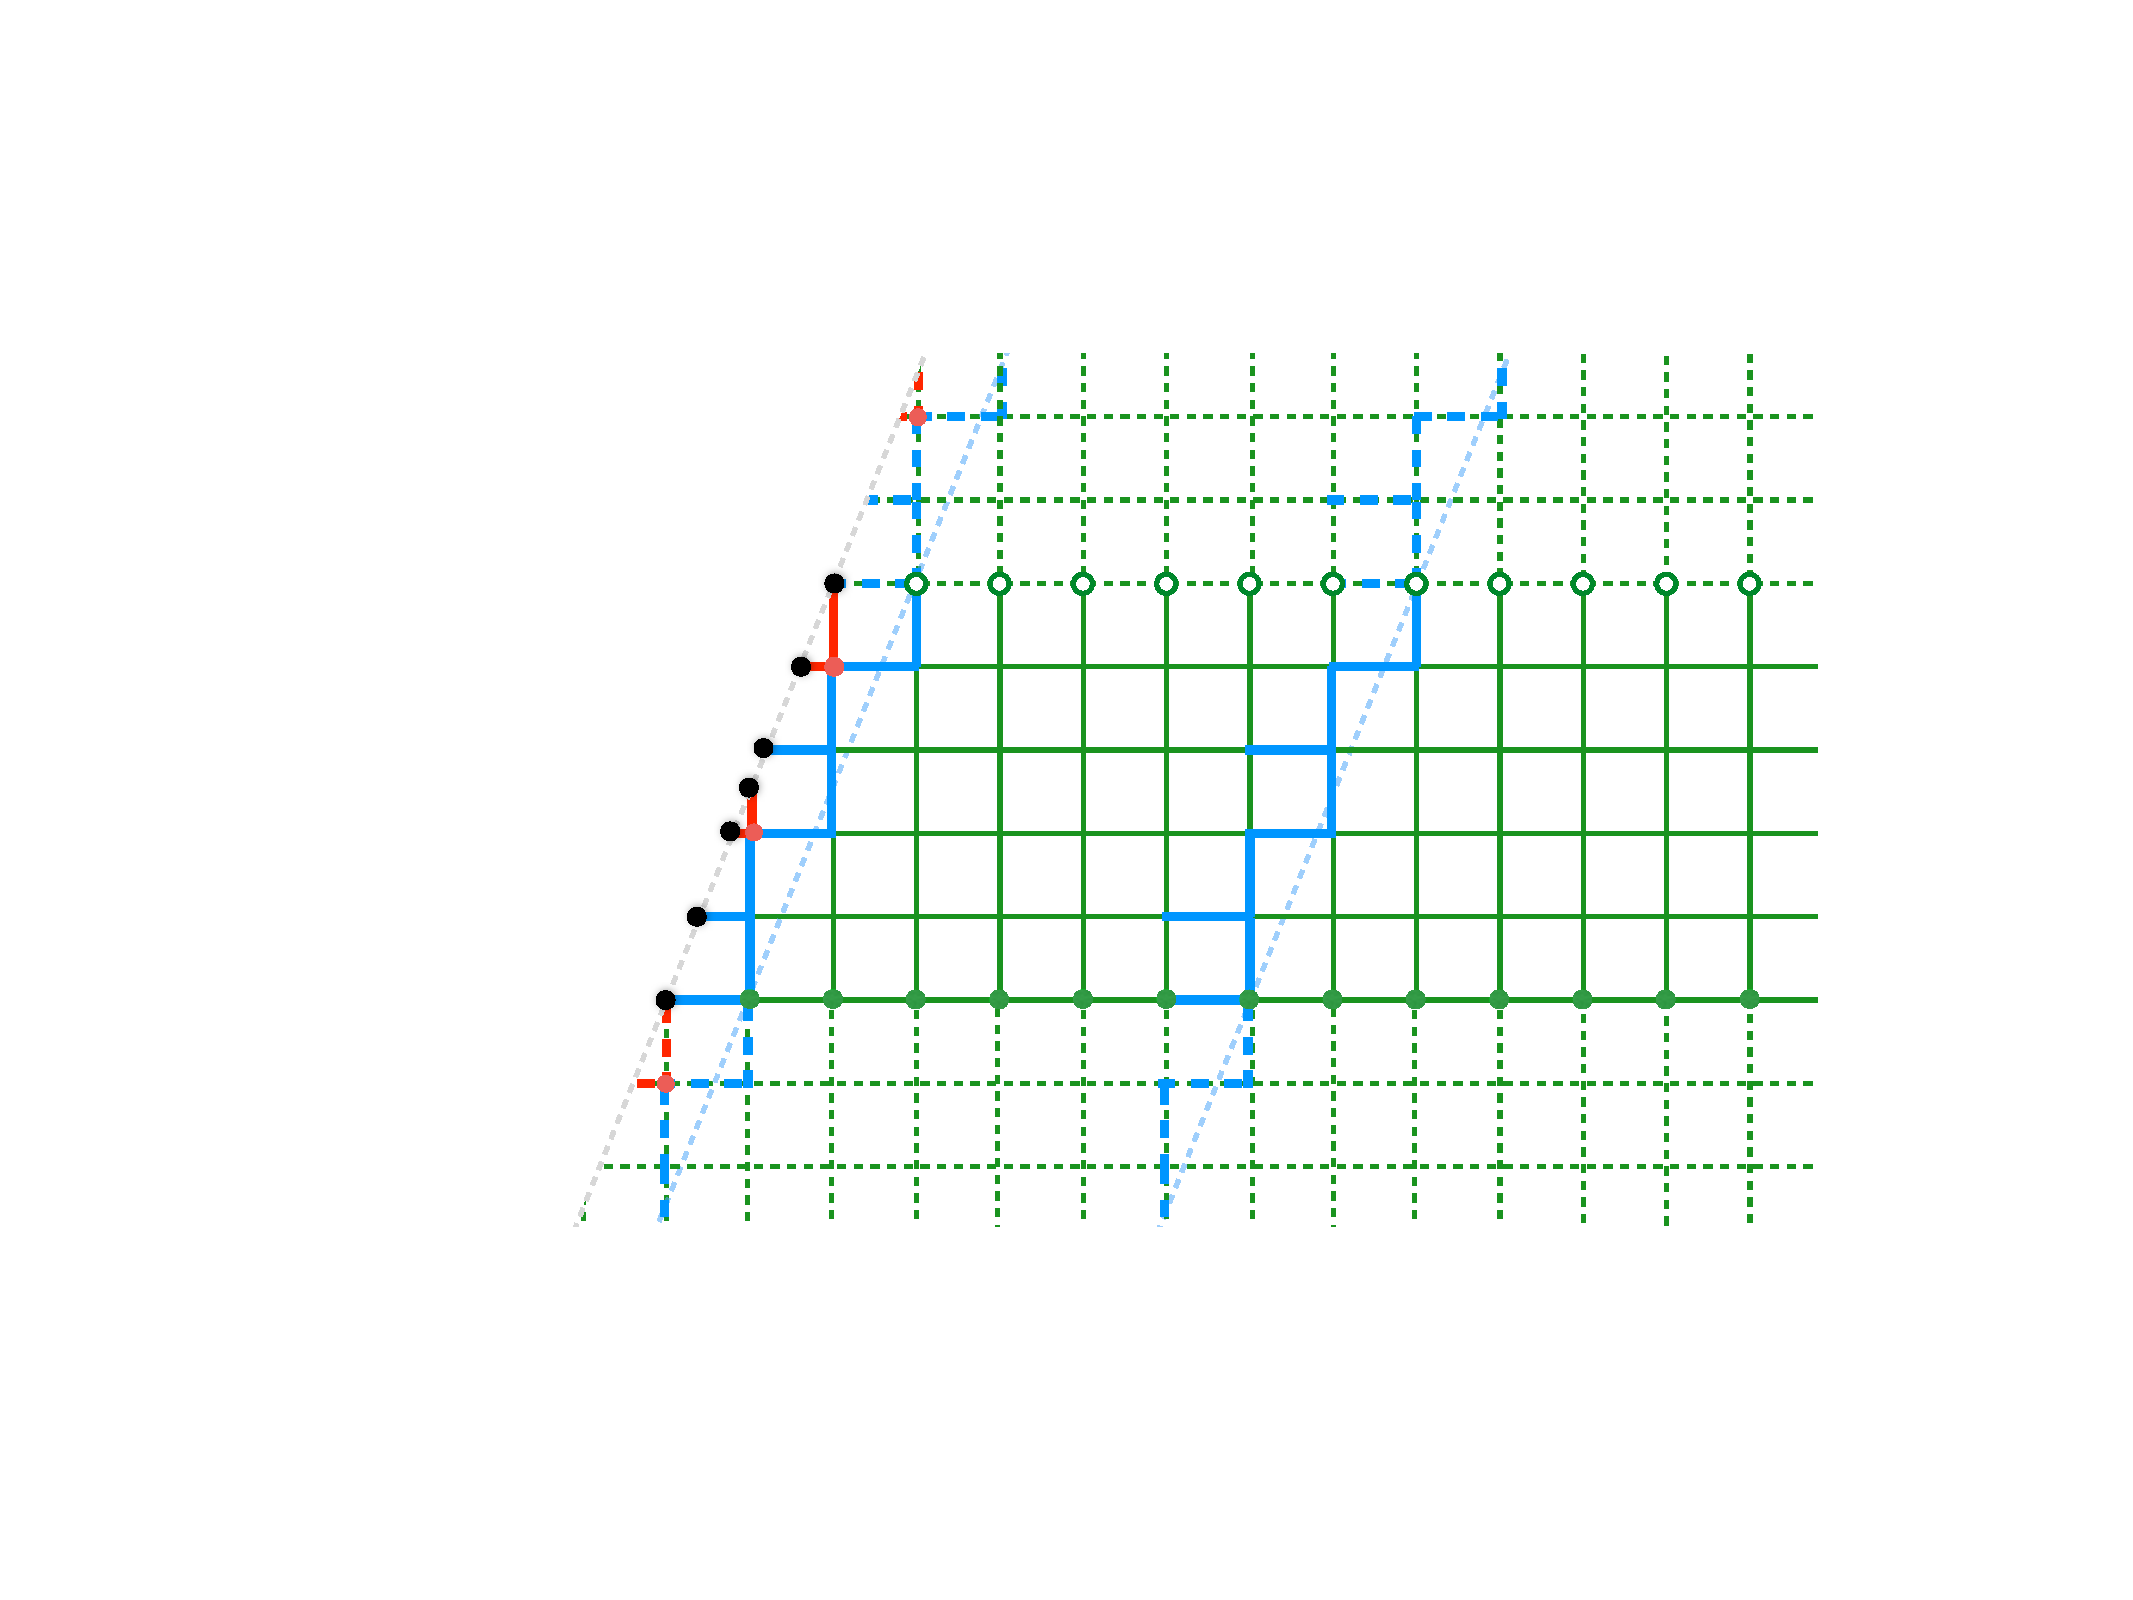
\includegraphics{Tube2.pdf}}
\caption{\small Forming a tube and a fundamental domain for shifts of the tube ...}
\label{fig:HalfTube}
\end{figure}



\begin{figure}   %%%%%%%%%%%%%%%%% FIGURE %%%%%%%%%%%%%%%%%%
\scalebox{0.36}{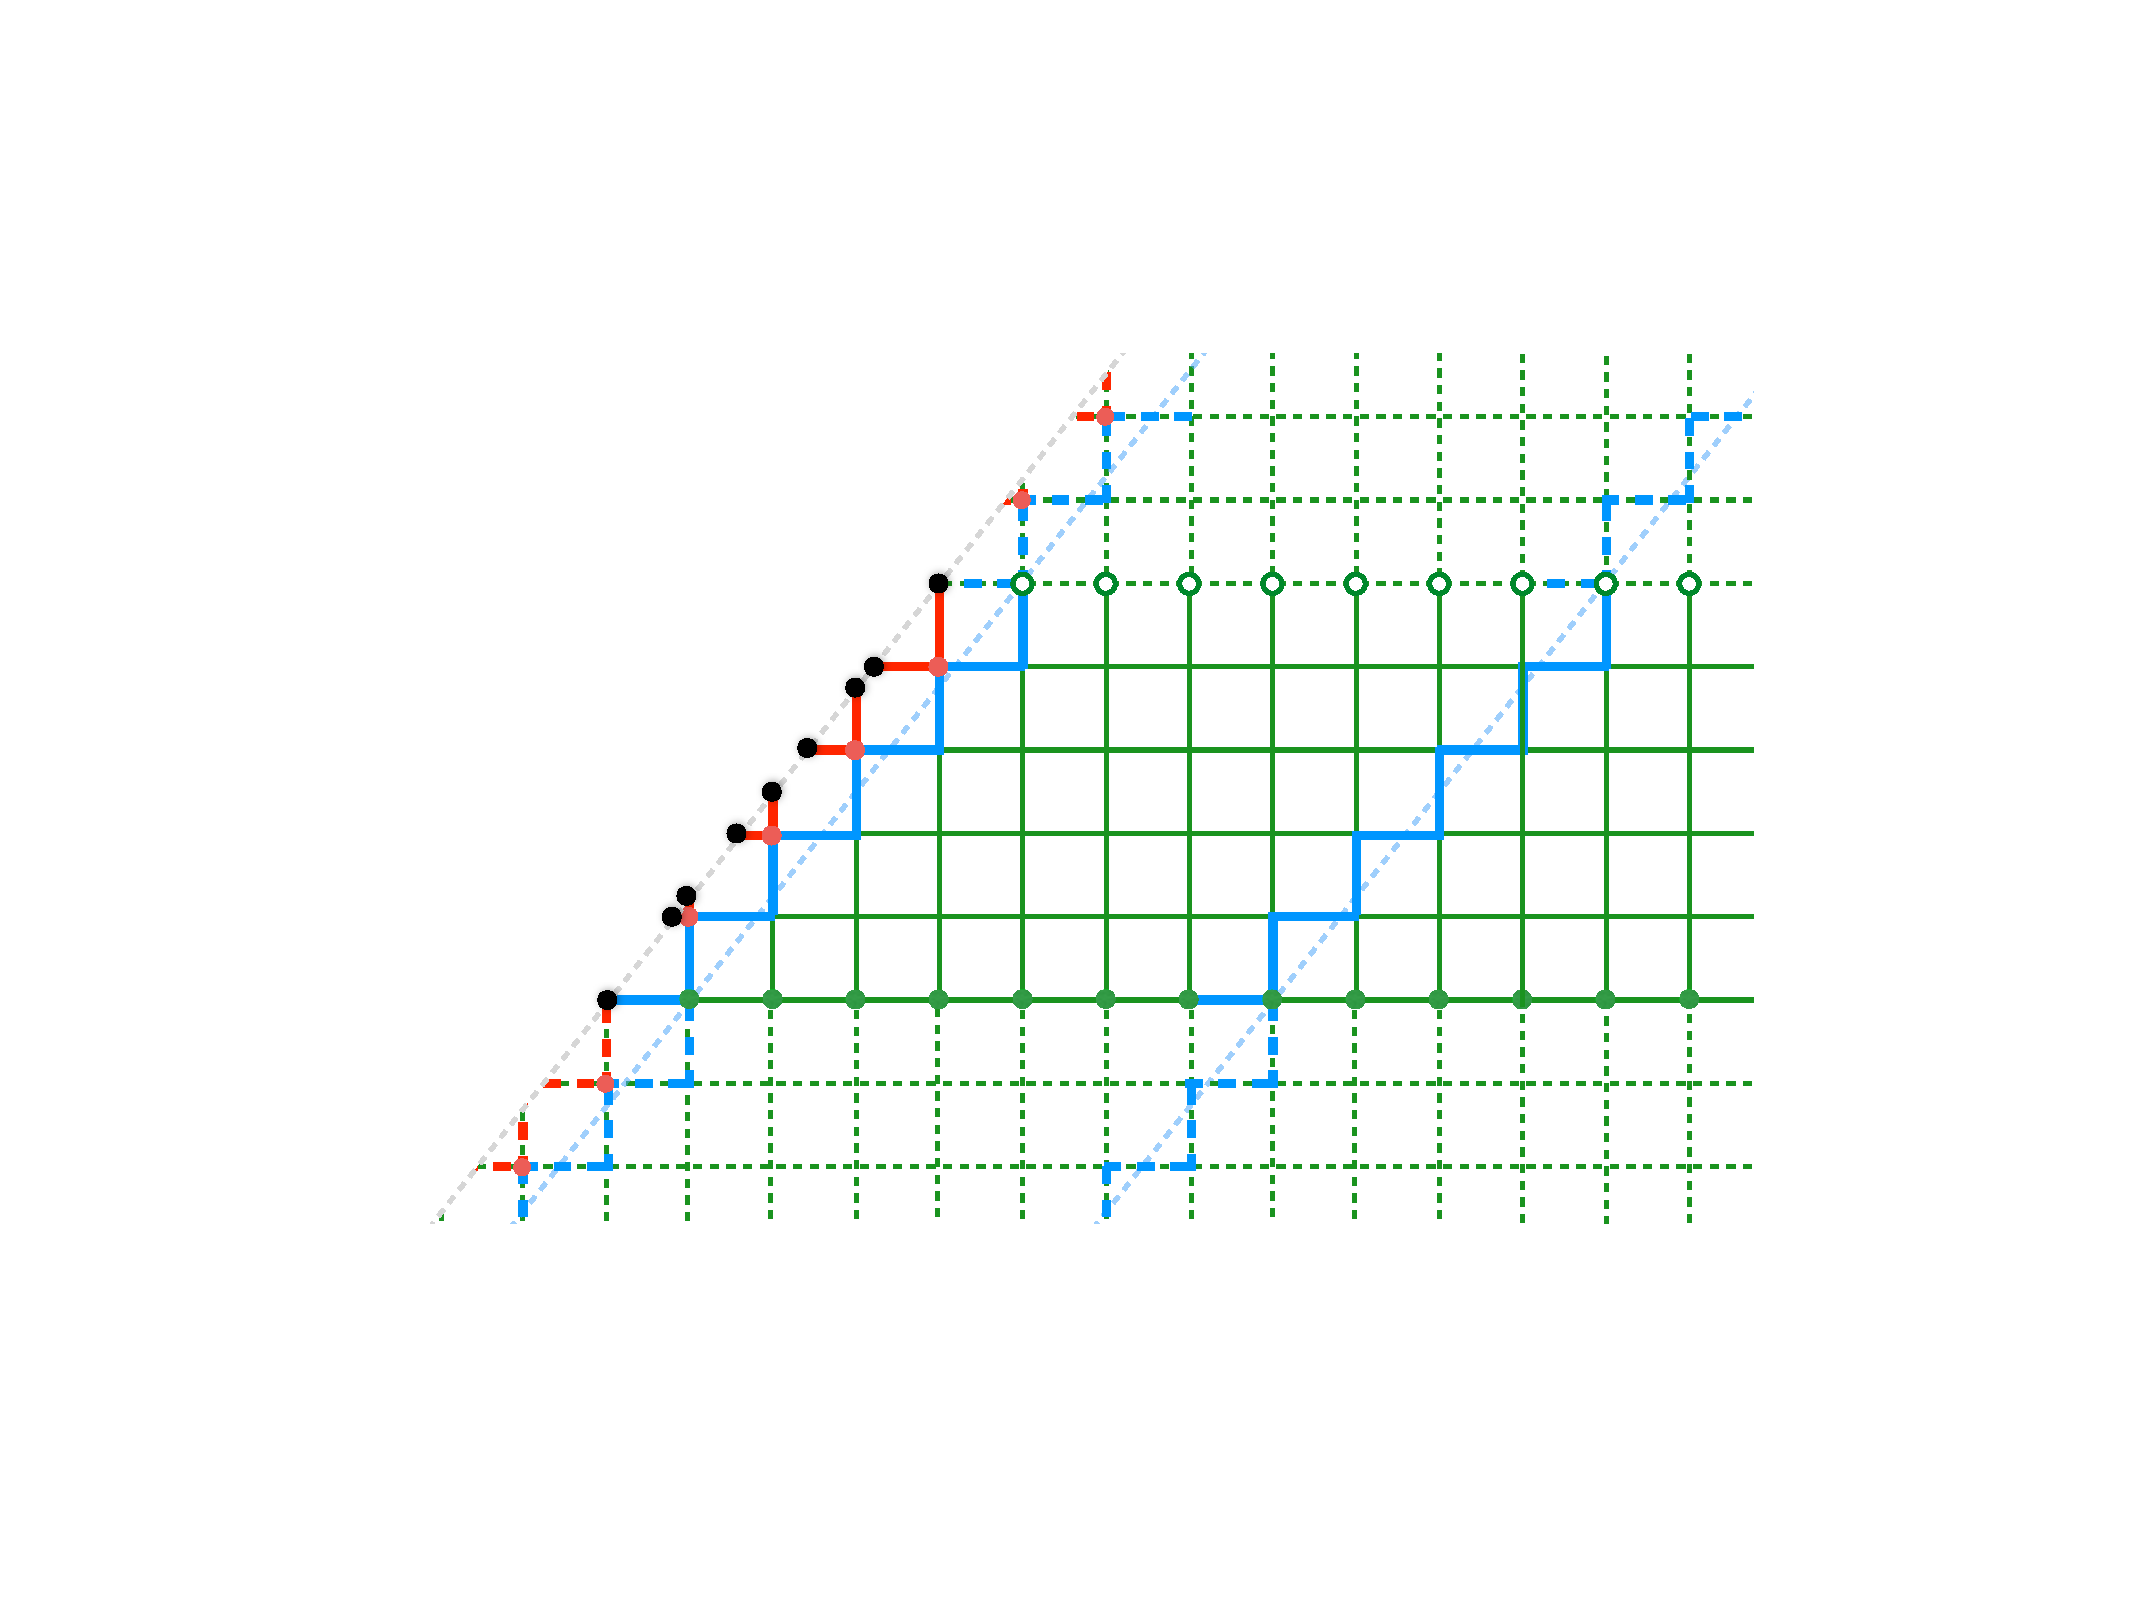
\includegraphics{Tube4.pdf}}
\hfill
\scalebox{0.36}{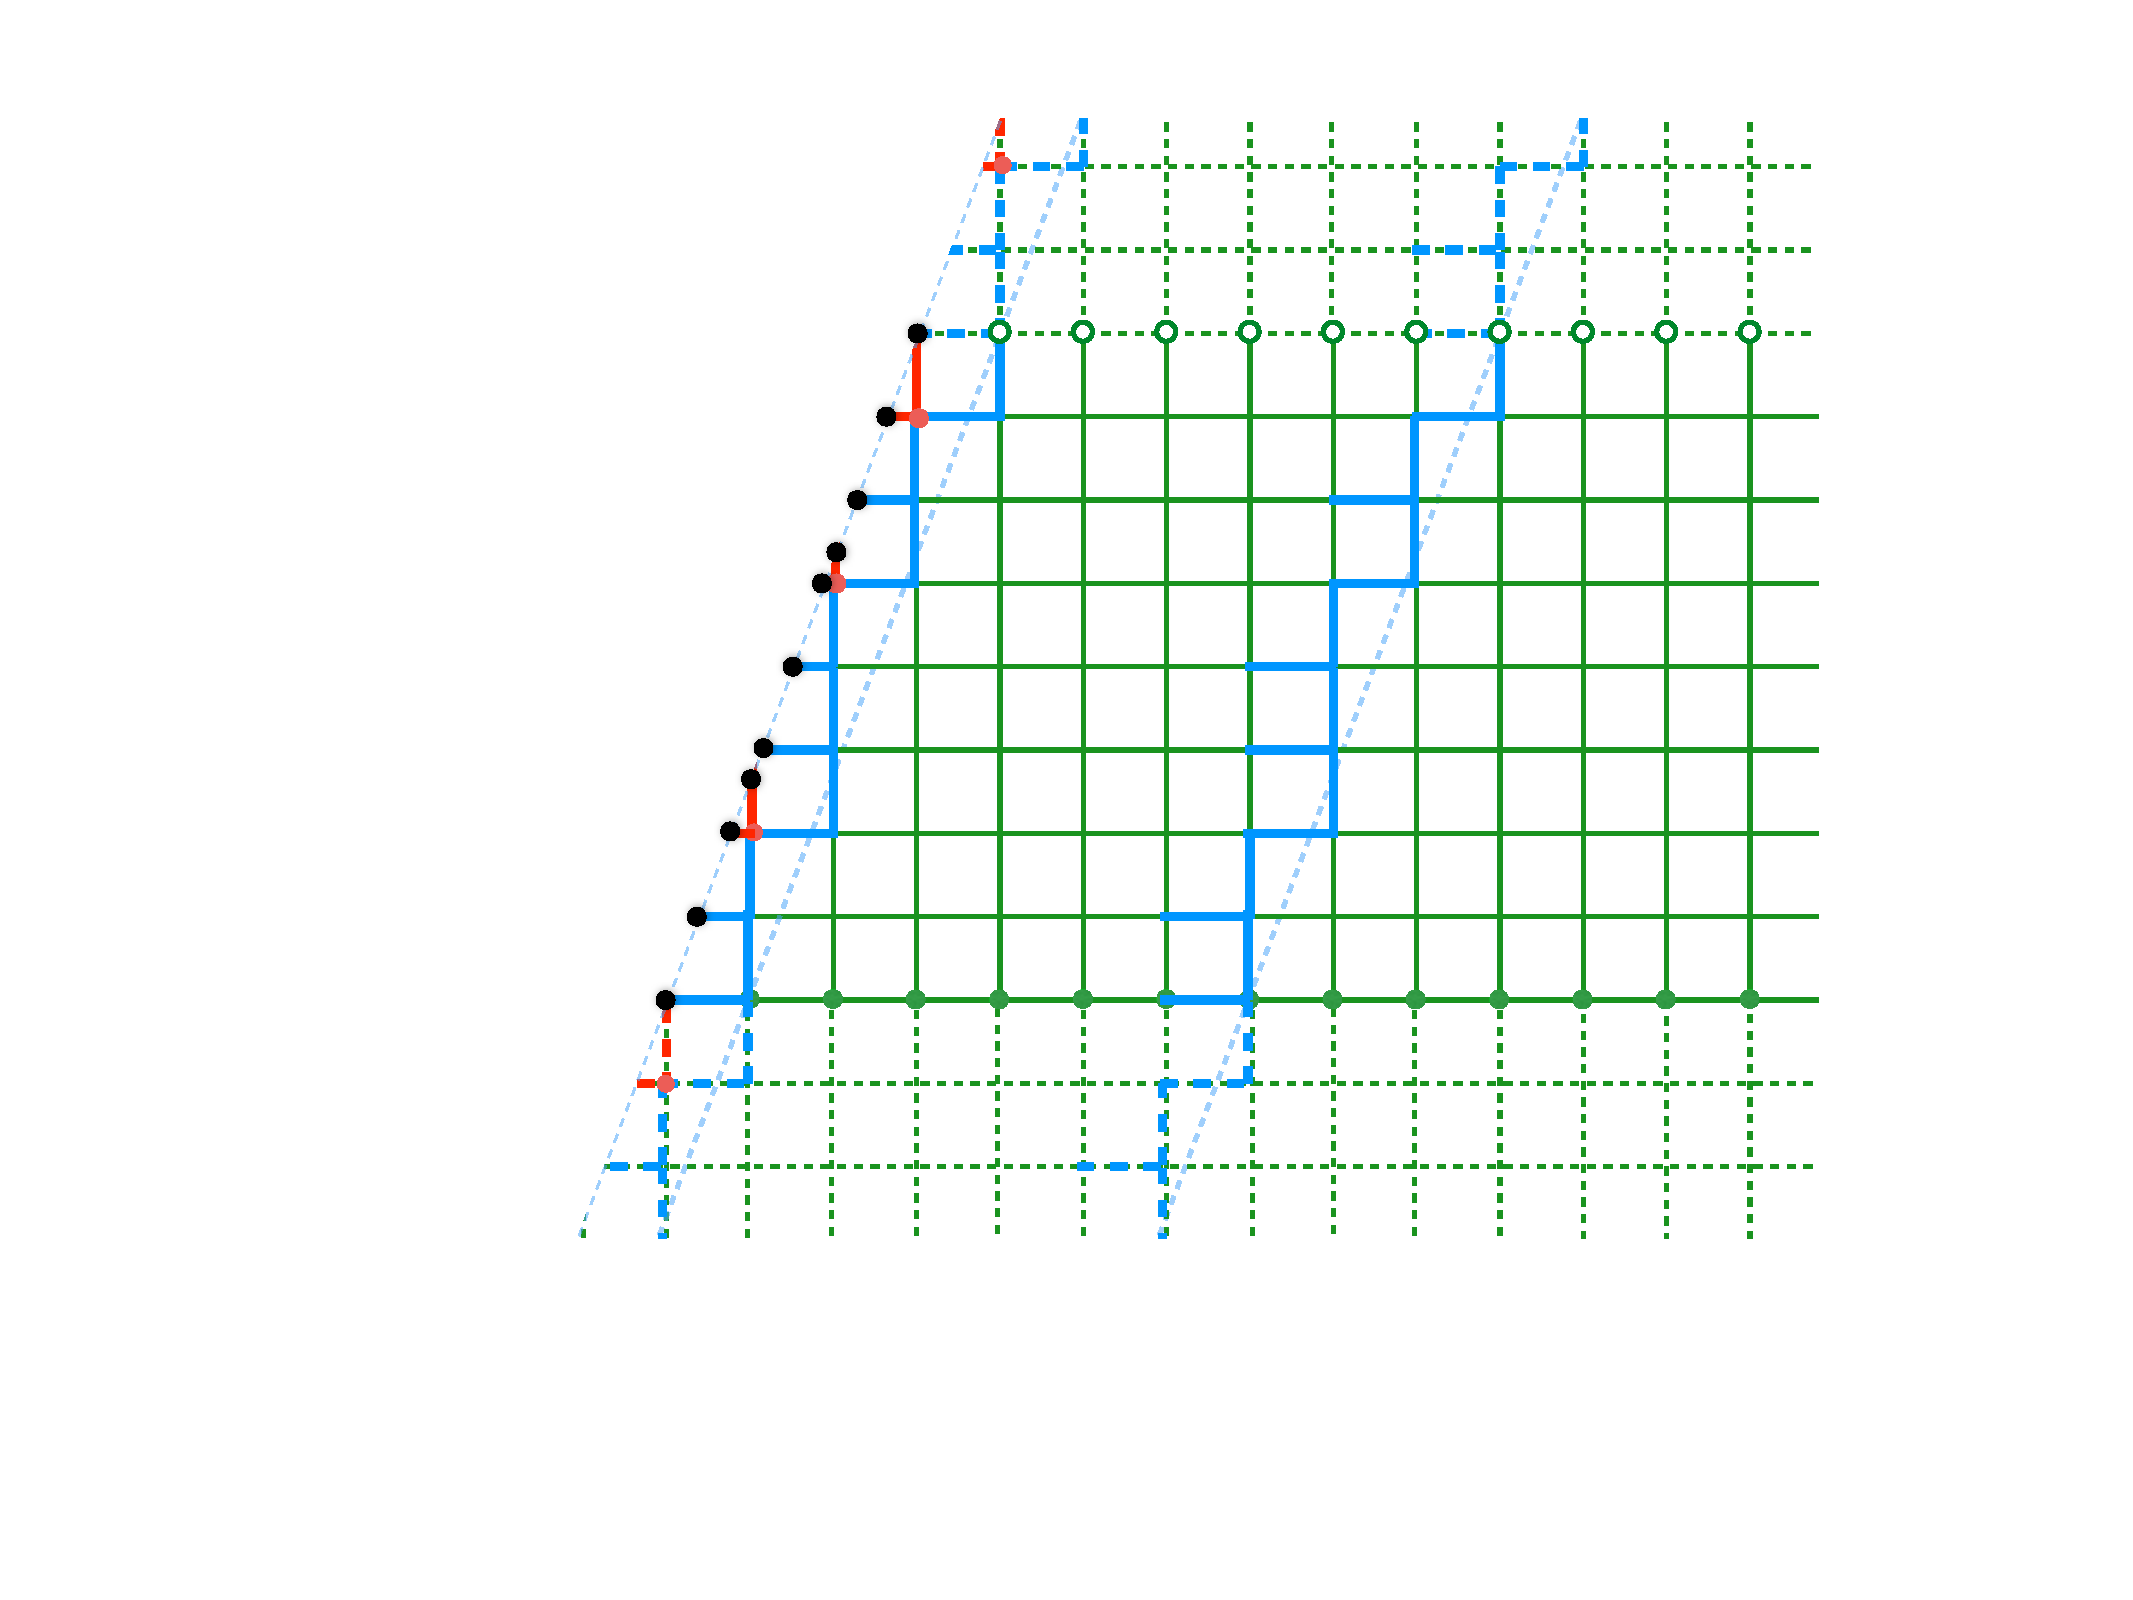
\includegraphics{Tube3.pdf}}
\caption{\small Two more examples of cutting the tube in half and the domains of the auxiliary boundary fields: $(\alpha,\beta)=(4,5)$ and $(\alpha,\beta)=(3,8)$.}
\label{fig:HalfTubes}
\end{figure}




\subsection{Self-adjoint boundary conditions}\label{sec:self-adjoint}  %%%%%%%%%%%
 
In order to make a Schr\"odinger operator on $T_+$ self-adjoint, appropriate functional conditions at the boundary vertices must be imposed.  Each set of self-adjoint conditions corresponds to a domain of functions that lies between a maximal domain $\Dmax\subset L^2(T_+)$, on which no boundary conditions are imposed, and a minimal domain $\Dmin\subset L^2(T_+)$, on which both the function and its derivative vanish at the boundary vertices:
%
\begin{equation}
\renewcommand{\arraystretch}{1.1}
\left.
\begin{array}{l}
    \Dmax = \left\{ u\in H^2(E(T_+)) :
            \text{$u$ satisfies the standard condition at internal vertices} \right\}\\
    \Dmin = \left\{ u\in \Dmax :
            \text{$u=0$ and $u'=0$ at the boundary vertices} \right\}.
\end{array}
\right.
\end{equation}
%
%In addition, define the domain
%
%\begin{equation}
%  \Dloc = \left\{ u\in \Hloc(E(T_+)) :
%            \text{$u$ continuous and satisfies zero-flux condition at internal vertices} \right\}
%\end{equation}
%

Let $\Hmax$ and $\Hmin$ denote the operator $-d^2/dx^2$ on the domains $\Dmax$ and $\Dmin$, respectively.
The minimal operator $H_-$ is symmetric with respect to the inner product in $L^2(T_+)$, and its adjoint is the maximal operator $H_+$:
%
\begin{eqnarray}
  && \langle H_- u, u \rangle = \langle u, H_- u \rangle \;\text{ for all}\; u\in\Dmin \\
  && (H_-)^* = H_+\,.
\end{eqnarray}
%
The eigenspaces
%
\begin{equation}
  \Nlambda := \{ u\in\Dmax : H_+ u = \lambda u \},
\end{equation}
%
especially the {\em deficiency spaces} $\Nplus$ and $\Nminus$, are central to the theory of self-adjoint extensions of the symmetric operator $H_-$ (see the classic~\cite{AkhiezerGlazman1993}, for example).

Theorem~\ref{thm:eigenspaces} states that the dimension of $\Nlambda$, when $\lambda$ is not real-valued, is equal to $\alpha+\beta$, and it identifies a natural basis for $\Nlambda$ consisting of the evanescent Floquet modes and certain {\itshape auxiliary boundary fields} localized on boundary edges.  More specifically, the values of an eigenfunction $u\in\Nlambda$ on any one translate of the domain $W$ (illustrated in blue in Figs.~\ref{fig:HalfTube} and \ref{fig:HalfTubes}) determine $u$ on all of $T_+$ except on $\alpha$ pairs of adjacent pendant edges at the boundary where the tube $T$ was cut.  These pairs of edges are illustrated in red in Figs.~\ref{fig:HalfTube} and \ref{fig:HalfTubes}, and are referred to as ``boundary frills".  The auxiliary boundary fields are functions $u\in\Dmax$ with support on the boundary frills.
%
Denote the boundary frills by $F_j$ for $1\leq j\leq \alpha$,
%
%\begin{equation}
%  \left\{ F_j \right\}_{j=1}^{\alpha}
%\end{equation}
%
where $F_j$ is ...
The space of auxiliary boundary fields is 
%
\begin{equation}
  \Daux := \left\{ u\in\Dmax \,:\, \supp(u) \,\subset\,\raisebox{-2pt}{\text{\Large$\cup$}}\! \left\{ F_j \right\}_{j=1}^{\alpha} \right\}.
\end{equation}
%


\begin{figure}   %%%%%%%%%%%%%%%%% FIGURE %%%%%%%%%%%%%%%%%%
\centerline{\scalebox{0.4}{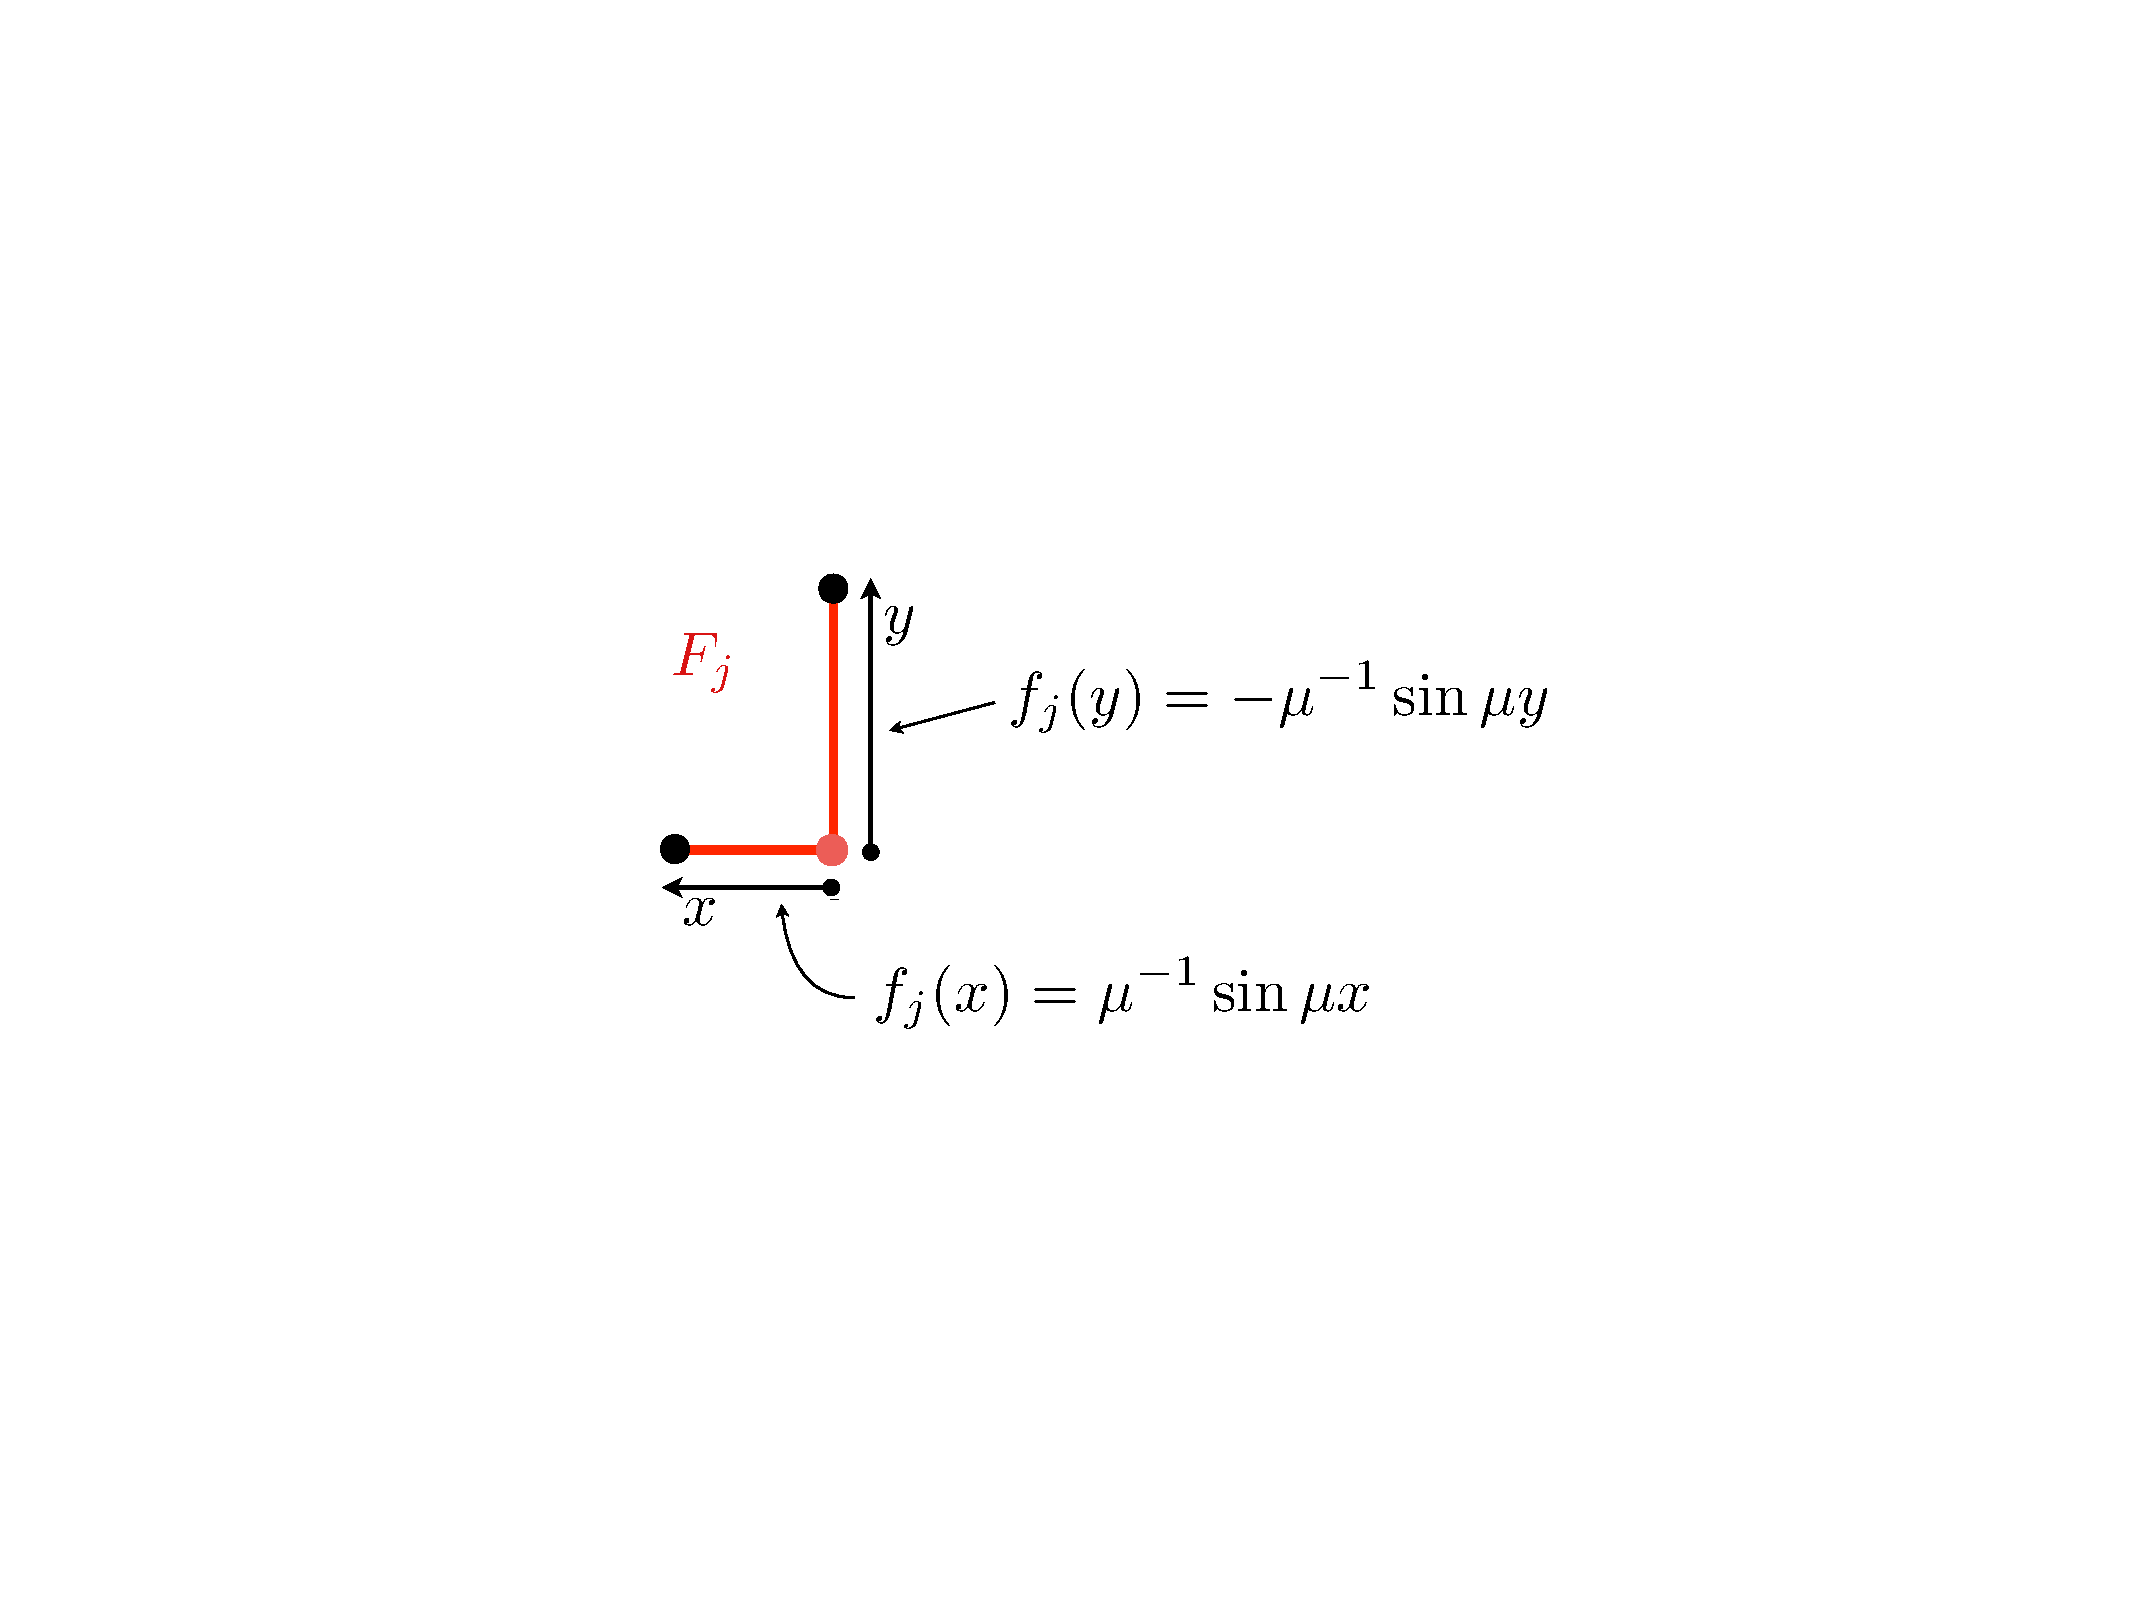
\includegraphics{Frill.pdf}}}
\caption{\small Boundary frills $F_j$ and auxiliary boundary fields $f_j$ ...}
\label{fig:Frill}
\end{figure}


Denote by $\Alambda$ the $\lambda$-eigenfunctions of $H_+$ that reside in $\Daux$:
%
\begin{equation}
  \Alambda := \Nlambda \cap \Daux
                   = \left\{ u\in\Daux : H_+u = \lambda u \right\}.
\end{equation}
%
The dimension of the space $\Alambda$ is $\alpha$, as stated in the following lemma, and a basis is constructed as follows.
  Given $\lambda\in\CC$ and $j:1\leq j\leq\alpha$, let the horizontal and vertical pendant edges of the frill $F_j$ be parameterized by variables $x$ and $y$, respectively, with the origins $x=0$ and $y=0$ located at the vertex $w_j$ that joins the two edges (Fig.\,\ref{fig:Frill}).  Define the function $f_j$ on $F_j$~by
%
\begin{equation}\label{fj}
  \renewcommand{\arraystretch}{1.1}
\left.
\begin{array}{ll}
    f_j(x) \,=\, \hspace{9pt}\mu^{-1} \sin \mu x  & \text{in the horizontal edge,} \\
    f_j(y) \,=\, - \mu^{-1} \sin \mu y  & \text{in the vertical edge,}
\end{array}
\right.
\end{equation}
%
where $\lambda=\mu^2$.  The square root branch cut taken along the negative real half-axis and $\mu>0$ for $\lambda>0$ and $\mu=i|\mu|$ for $\lambda<0$.  For $\mu=0$, (\ref{fj}) is understood as the limit as $\mu\to0$, so that $f_j(x)=x$ and $f_j(y)=-y$ on the respective edges. 

\begin{lemma}\label{lemma:Alambda}  %%%%%%%%%%% LEMMA %%%%%%%%%%%%
The ordered set
%
%\begin{equation}
  $\{ f_j \}_{j=1}^\alpha$
%\end{equation}
%
is a basis for the space $\Alambda$.
\end{lemma}

\begin{proof}
  proof
\end{proof}

\begin{lemma}\label{lemma:eigenspaces}  %%%%%%%%%%% LEMMA %%%%%%%%%%%%
Let $g\in\ZZ$ be such that the h-translate $gW$ of $W$ is contained entirely in $T_+$.

\smallskip
(a.\,existence) Let a function $\tilde u\in H^2_*(gW)$ \notesps{define} satisfy $H\tilde u=\lambda \tilde u$ \notesps{make sure $H$ makes sense on such general domains} and the \notesps{...} vertex conditions at each internal vertex of $gW$.  Then there exists an extension $u\in H^2_*(T_+)$ of $\tilde u$ such that $Hu=\lambda u$. 

\smallskip
(b.\,almost uniqueness) Suppose that $\lambda\not\in\sigma_D$, and that $u$ and $v$ are functions in $\Hloc(T_+)$ such that $H u = \lambda u$ and $H v = \lambda v$ and that $u$ and $v$ coincide on $gW$, that is,
%
\begin{equation}
  u(p) = v(p) 
  \qquad
  \text{for all}
  \qquad
  p \in g W.
\end{equation}
%
Then $u$ and $v$ coincide on all of $T_+$ except on the boundary frills, that is,
%
\begin{equation}
  u(p) = v(p) 
  \qquad
  \text{for all}
  \qquad
  p \in T_+ \setminus \raisebox{-2pt}{\text{\Large$\cup$}} \left\{ F_j \right\}_{j=1}^\alpha\,.
\end{equation}
%
\end{lemma}

\begin{proof}
    ... appeal to Theorem~\ref{thm:modes} ...

  (a) ... standard extension by extending uniquely to $T$ and then restricting to $T_+$ ...
  
  (b) ... previous shows uniqueness in each translation $hW$ that lies entirely in $T_+$, and thus $u-v$ vanishes everywhere in $T_+$, except for possibly on the boundary frills $F_j$, $1\leq j\leq\alpha$. ...
  
\end{proof}


  %%%%%%%%%%% THEOREM %%%%%%%%%%%%
\begin{theorem}[Eigenspaces of $H_+$]\label{thm:eigenspaces} 
  Theorem on dimension and basis for $\Nlambda$.
\end{theorem}

\begin{proof}
  Proof.
    ... appeal to Theorem~\ref{thm:modes} ...
\end{proof}



\subsection{Reflection from the boundary}\label{sec:reflection} %%%%%%%%%%%





\bigskip
... the boundary data $(F,F')$ and reparsed data
%
\begin{eqnarray}
  G^+ &=& F + iF' = (1-\mu) G^\text{p} + (1+\mu) G^\text{n}, \\
  G^- &=& F - iF' = (1+\mu) G^\text{p} + (1-\mu) G^\text{n},
\end{eqnarray}
%
in which $G^\text{p}$ and $G^\text{n}$ are defined using the decomposition of the numbers $j\alpha/\beta$ and $j\beta/\alpha$ into their integer and remainder parts:
%
\begin{eqnarray}
  \alpha\frac{j}{\beta} = p_{1j} + \frac{\hat j_{1j}}{\beta}, && 0\leq j<\beta \\
  \beta\frac{j}{\alpha} = p_{2j} + \frac{\hat j_{2j}}{\alpha}, && 0\leq j<\alpha  
\end{eqnarray}
%
and reference to Fig...
%
\begin{equation}
  G^\text{p} \,=\,
\renewcommand{\arraystretch}{1.4}
\left[
  \begin{array}{l}
    \{ \textstyle \left( z^\beta e^{i\mu x} - e^{i\mu(x-1)} \right) z^{\beta p_{1j}} \,:\, x=\frac{\hat j_{1j}}{\beta},\; 0\leq j<\beta \} \\
    \{ \textstyle \left( \eta z^\alpha e^{i\mu x} - e^{i\mu(x-1)} \right) (\eta z^\alpha)^{p_{2j}} \,:\, x=\frac{\hat j_{2j}}{\alpha},\; 0\leq j<\alpha \}    
  \end{array}
\right]
\end{equation}
%
and
%
\begin{equation}
  G^\text{n} \,=\,
\renewcommand{\arraystretch}{1.4}
\left[
  \begin{array}{l}
    \{ \textstyle \left( z^\beta e^{-i\mu x} - e^{-i\mu(x-1)} \right) z^{\beta p_{1j}} \,:\, x=\frac{\hat j_{1j}}{\beta},\; 0\leq j<\beta \} \\
    \{ \textstyle \left( \eta z^\alpha e^{-i\mu x} - e^{-i\mu(x-1)} \right) (\eta z^\alpha)^{p_{2j}} \,:\, x=\frac{\hat j_{2j}}{\alpha},\; 0\leq j<\alpha \}    
  \end{array}
\right]
\end{equation}
%




\subsection{Bound states for the half-tube}\label{sec:boundstates} %%%%%%%%%%%







\bigskip

Temporary citations:
\cite{BerkolaikoKuchment2013,KuchmentPost2007,Shipman2014}



\bibliography{QGTubes}

\end{document}
























